\documentclass[12pt, a4paper, oneside, openany]{report}

% PAQUETES ESSENCIALES
\usepackage[spanish]{babel}
\usepackage[left=2cm, right=2cm, top=2cm, bottom=2cm]{geometry}
\usepackage{graphicx}
\usepackage{booktabs}
\usepackage{multirow}
\usepackage{amsmath}
\usepackage{amssymb}
\usepackage{float}
\usepackage{hyperref}
\usepackage{listings}
\usepackage{xcolor}
\usepackage{fancyhdr}
\usepackage{tocbibind}
\usepackage{caption}
\usepackage{subcaption}
\usepackage{tikz}
\usepackage{rotating}
\usepackage{color}

% CONFIGURACION DE ESTILOS
\pagestyle{fancy}
\fancyhead[L]{\small\nouppercase{\leftmark}}
\fancyhead[R]{\small\thepage}
\fancyfoot[C]{}
\renewcommand{\footrulewidth}{0pt}
\renewcommand{\headrulewidth}{0.4pt}

% COLORES PARA LATEX
\definecolor{darkblue}{rgb}{0, 0, 0.5}
\definecolor{darkgreen}{rgb}{0, 0.4, 0}
\definecolor{darkred}{rgb}{0.6, 0, 0}

% CONFIGURACION DE HIPERVINCULOS
\hypersetup{
    colorlinks=true,
    linkcolor=darkblue,
    filecolor=darkblue,
    urlcolor=darkblue,
    citecolor=darkblue,
    pdftitle={FatigueSet Dataset - Documentacion Completa},
    pdfauthor={TFG - Analisis de Fatiga Multimodal},
    pdfsubject={Dataset FatigueSet}
}

% CONFIGURACION DE CODIGO
\lstset{
    basicstyle=\ttfamily\small,
    breaklines=true,
    frame=single,
    numbers=left,
    numberstyle=\tiny,
    keywordstyle=\color{darkblue}\bfseries,
    commentstyle=\color{darkgreen},
    stringstyle=\color{darkred},
    language=Python,
    showstringspaces=false,
    tabsize=2,
    captionpos=b
}

% ESPACIADO
\renewcommand{\baselinestretch}{1.05}
\setlength{\parindent}{0.5cm}
\setlength{\parskip}{0.15cm}

% TITULO Y AUTOR
\title{\Huge \textbf{FatigueSet:\\Documentacion Completa del Dataset}}
\author{\textit{Dataset Multimodal para Modelado de Fatiga Mental y Fisica}\\[0.5cm]
        \small{Basado en: Kalanadhabhatta et al. (2021)\\
        Pervasive Health Conference}
        }
\date{\today}

% ============================================================
% INICIO DEL DOCUMENTO
% ============================================================

\begin{document}

% PORTADA
\maketitle

% RESUMEN EJECUTIVO
\begin{abstract}
\noindent
Este documento proporciona una explicacion completa y detallada del dataset FatigueSet,
un dataset multimodal disenado para estudiar fatiga mental y fisica en seres humanos.

El dataset contiene datos de 12 participantes en 3 sesiones experimentales cada uno,
con mediciones de 4 dispositivos wearables simultaneamente (Nokia Bell Labs eSense,
Muse S Headband, Zephyr BioHarness 3.0 y Empatica E4), junto con tareas cognitivas
estandarizadas y autoreportes de fatiga.

Se explica en detalle:
\begin{itemize}
    \item La estructura y protocolo experimental del estudio
    \item Las especificaciones tecnicas de cada sensor wearable
    \item Las tareas cognitivas y metricas comportamentales recopiladas
    \item Las 19 variables fisiologicas agregadas del dataset
    \item Analisis cuantitativos con 14 visualizaciones
    \item Patrones de fatiga observados en los datos
    \item Como utilizar el dataset en investigaciones propias
\end{itemize}

La audiencia objetivo incluye investigadores, estudiantes y profesionales
que necesiten un entendimiento integral del dataset.
\end{abstract}

\newpage

% TABLA DE CONTENIDOS
\tableofcontents

\newpage

% ============================================================
% CAPITULOS
% ============================================================

\chapter{Introduccion}
\label{cap:introduction}

\section{Contexto: Fatiga Mental y Fisica}

La fatiga es un estado fisiologico y psicologico complejo que afecta significativamente
el rendimiento cognitivo, la capacidad fisica y la calidad de vida. En contextos
academicos, laborales y deportivos, entender y medir la fatiga es crucial para
optimizar el desempenho y prevenir problemas de salud.

La fatiga se puede clasificar en dos categorias principales:

\begin{itemize}
    \item \textbf{Fatiga Fisica}: Cansancio o agotamiento muscular resultante del
          esfuerzo fisico intenso o prolongado. Se asocia con cambios en el metabolismo,
          acumulacion de lactato y deplecion de glucogeno.

    \item \textbf{Fatiga Mental}: Cansancio cognitivo resultante de la concentracion
          prolongada o tareas cognitivamente demandantes. Se asocia con cambios en
          actividad cerebral, control ejecutivo y vigilancia.
\end{itemize}

\section{Importancia del Monitoreo Multimodal}

Durante decadas, los investigadores han intentado entender la fatiga mediante
distintos enfoques:

\begin{enumerate}
    \item \textbf{Mediciones Subjetivas}: Cuestionarios y escalas de autopercepcion
          (ej: Escala Visual Analogica de Fatiga). Ventaja: economicas. Desventaja:
          susceptibles a sesgo y variabilidad individual.

    \item \textbf{Mediciones Fisiologicas Aisladas}: Frecuencia cardiaca,
          electroencefalograma (EEG), o respuesta electrodermal medidas
          independientemente. Ventaja: objetivas. Desventaja: incompletas.

    \item \textbf{Monitoreo Multimodal Simultaneo}: Multiples sensores wearables
          registrando simultaneamente diferentes variables fisiologicas, comportamentales
          y cognitivas. Ventaja: comprensiva, registra interacciones entre sistemas.
          Desventaja: mayor complejidad de analisis.
\end{enumerate}

El enfoque multimodal es particularmente importante porque la fatiga no es un
fenomeno unidimensional. Por ejemplo:

\begin{itemize}
    \item La frecuencia cardiaca puede aumentar o disminuir segun el tipo y
          intensidad de actividad y el estado cardiovascular del individuo.
    \item La actividad electrodermal refleja arousale (activacion del sistema nervioso
          simpatico) pero puede estar influenciada por factores emocionales o
          termicos.
    \item La actividad cerebral (EEG) proporciona informacion sobre estados cognitivos
          (alerta vs. somnolencia) pero requiere interpretacion cuidadosa de bandas
          de frecuencia.
\end{itemize}

Al monitorear multiples modalidades simultaneamente, podemos:
\begin{itemize}
    \item Detectar \textbf{patrones complejos} que emergen de la interaccion entre sistemas
    \item \textbf{Validar hallazgos} comparando senales independientes
    \item Desarrollar \textbf{modelos predictivos} mas robustos y generalizables
    \item Identificar \textbf{diferencias individuales} en como cada persona manifiesta la fatiga
\end{itemize}

\section{FatigueSet: Su Importancia en la Investigacion}

Aunque existen datasets de EEG, de actividad cardiaca, o de tareas cognitivas de
forma aislada, los datasets verdaderamente multimodales y accesibles publicamente
son escasos. FatigueSet llena este vacio proporcionando:

\begin{itemize}
    \item Una \textbf{recopilacion completa} de 4 dispositivos wearables de marcas
          comerciales diferentes pero bien documentadas
    \item Un \textbf{protocolo experimental riguroso} con contrabalanceo para
          investigar fatiga a multiples intensidades
    \item \textbf{Tareas cognitivas estandarizadas} (CRT, N-Back, Task Switching)
          junto con autoreportes validados
    \item \textbf{Datos procesados y limpios} listos para analisis, junto con codigo
          y documentacion
\end{itemize}

Este dataset ha permitido y seguira permitiendo investigacion en:
\begin{itemize}
    \item Deteccion automatica de fatiga mediante machine learning
    \item Entendimiento de mecanismos fisiologicos subyacentes a fatiga mental vs fisica
    \item Individualizacion de perfiles de respuesta a fatiga
    \item Validacion de nuevos sensores wearables
    \item Estudios de recuperacion y resilencia ante fatiga
\end{itemize}

\section{Objetivos de Este Documento}

Este documento tiene como objetivo proporcionar una referencia completa y autocontenida
del dataset FatigueSet. No asume conocimiento previo del dataset pero mantiene
rigor academico y tecnico.

Despues de leer este documento, el lector podra:

\begin{enumerate}
    \item Comprender la estructura general del estudio que genero el dataset
    \item Identificar que dispositivo recopilo que tipo de senales
    \item Interpretar cada una de las 19 variables fisiologicas disponibles
    \item Entender los patrones de fatiga observados en los datos
    \item Cargar y utilizar el dataset en sus propios analisis
    \item Reproducir los analisis mostrados en este documento
\end{enumerate}

\section{Estructura de Este Documento}

El documento esta organizado en 8 capitulos progresivos:

\begin{description}
    \item[Capitulo 1] (Este capitulo) - Motivacion y contexto
    \item[Capitulo 2] - Vision general del dataset y protocolo experimental
    \item[Capitulo 3] - Los 4 dispositivos wearables utilizados
    \item[Capitulo 4] - Las 5 tareas cognitivas y metricas conductuales
    \item[Capitulo 5] - Las 19 variables fisiologicas extraidas (enfoque en patrones de fatiga)
    \item[Capitulo 6] - Analisis cuantitativos y 14 visualizaciones de datos
    \item[Capitulo 7] - Interpretacion de hallazgos y signos de fatiga
    \item[Capitulo 8] - Guia practica para utilizar el dataset
\end{description}

Los apendices incluyen especificaciones tecnicas completas, instrumentos de encuesta,
codigo de ejemplo y un glosario de terminos fisiologicos y tecnicos.

\chapter{Vision General del Dataset}
\label{cap:overview}

\section{Caracteristicas Principales}

El dataset FatigueSet contiene datos fisiologicos y comportamentales de
\textbf{12 participantes} que realizaron un protocolo experimental estructurado
para inducir fatiga mental y fisica controlada. Los datos fueron recopilados
en \textbf{3 sesiones} por participante, y cada sesion se dividio en
\textbf{3 fases de medicion}.

Las dimensiones principales del dataset son:

\begin{table}[H]
\centering
\caption{Dimensiones principales del FatigueSet}
\begin{tabular}{|l|r|p{5cm}|}
\hline
\textbf{Dimension} & \textbf{Valor} & \textbf{Notas} \\
\hline
Participantes & 12 & Etiquetados P01 a P12 \\
\hline
Sesiones por participante & 3 & Sesiones 01, 02, 03 \\
\hline
Fases de medicion por sesion & 3 & M1, M2, M3 \\
\hline
Dispositivos simultaneos & 4 & Wearables (ver Cap. 3) \\
\hline
Tareas cognitivas & 5 & CRT, N-Back, Task Switch, Fatigue Scale, Markers \\
\hline
Variables fisiologicas agregadas & 19 & HR, BR, HRV, EDA, EEG, etc. \\
\hline
Reglas de combinacion total & 12 x 3 x 3 & 108 registros en archivo agregado \\
\hline
\end{tabular}
\end{table}

\section{Protocolo Experimental y Contrabalanceo}

\subsection{Intensidad de Actividad}

Cada sesion fue disenada para inducir un nivel diferente de fatiga fisica:

\begin{itemize}
    \item \textbf{Low Intensity}: Actividad fisica ligera (caminar lentamente o
          ejercicio estatico suave). Induce minimo esfuerzo y fatiga.

    \item \textbf{Medium Intensity}: Actividad fisica moderada (ejercicio cardiovascular
          moderado). Induce fatiga moderada pero sostenible.

    \item \textbf{High Intensity}: Actividad fisica vigorosa (ejercicio intenso o HIIT-style).
          Induce fatiga aguda pronunciada.
\end{itemize}

\subsection{Contrabalanceo de Orden}

Para evitar efectos del orden (aprendizaje, fatiga acumulada entre sesiones),
los participantes fueron asignados a \textbf{ordenes contrabalanceados} de intensidad.
Por ejemplo:

\begin{table}[H]
\centering
\caption{Ejemplo de contrabalanceo (P01)}
\begin{tabular}{|c|c|c|c|}
\hline
\textbf{Participante} & \textbf{Sesion 1} & \textbf{Sesion 2} & \textbf{Sesion 3} \\
\hline
P01 & Low (1) & Medium (2) & High (3) \\
P02 & Low (1) & High (3) & Medium (2) \\
P03 & Medium (2) & High (3) & Low (1) \\
P04 & High (3) & Medium (2) & Low (1) \\
\vdots & \vdots & \vdots & \vdots \\
\hline
\end{tabular}
\end{table}

Este contrabalanceo de cuadrado latino asegura que no hay confusiones sistematicas
entre orden de sesion e intensidad de actividad.

\section{Tres Fases de Medicion: M1, M2, M3}

Dentro de cada sesion, el protocolo incluyo \textbf{tres fases temporales} donde
se recopilaron mediciones de todos los sensores:

\begin{description}
    \item[M1 - Baseline (Linea Base)]
    Duracion: ~10 minutos. El participante se encuentra en reposo, se sincroniza
    la instrumentacion, se recopilan mediciones EEG basales (ojos abiertos y cerrados).
    Esta fase sirve de comparacion para detectar cambios inducidos por la actividad.

    \item[M2 - Post-Ejercicio]
    Duracion: ~5-20 minutos (variable segun la intensidad de la actividad previa).
    Inmediatamente despues de completar la actividad fisica designada. Es la fase
    donde se observan cambios mas marcados en variables cardiovasculares y electrodermal.

    \item[M3 - Post-Fatiga Mental]
    Duracion: ~10 minutos. Despues de un bloque de tareas cognitivas (CRT, N-Back, Task Switch).
    Permite evaluar fatiga mental e interacciones entre fatiga fisica y mental.
\end{description}

Durante cada fase, los participantes completaron:
\begin{itemize}
    \item \textbf{Escala de Fatiga Subjetiva} (exp\_fatigue.csv) - 2 preguntas (fisica y mental)
    \item \textbf{Tareas Cognitivas} (exp\_crt.csv, exp\_nback.csv, exp\_task\_switch.csv)
    \item \textbf{Recopilacion de Datos Fisiologicos} - 4 dispositivos simultaneamente
\end{itemize}

\section{Estructura de Archivos}

El dataset esta organizado jerarquicamente:

\begin{verbatim}
fatigueset/
├── metadata.csv                          (Informacion de contrabalanceo)
├── 01/ 02/ ... 12/                       (Directorios por participante)
│   ├── 01/ 02/ 03/                       (Subdirectorios por sesion)
│   │   ├── exp_crt.csv                   (Tarea CRT)
│   │   ├── exp_nback.csv                 (Tarea N-Back)
│   │   ├── exp_task_switch.csv           (Tarea Task Switch)
│   │   ├── exp_fatigue.csv               (Escala de fatiga subjetiva)
│   │   ├── exp_markers.csv               (Marcadores temporales)
│   │   ├── ear_acc_left.csv, ...         (Nokia eSense - 6 archivos)
│   │   ├── forehead_eeg_alpha_abs.csv, ...(Muse S - 13 archivos)
│   │   ├── chest_physiology_summary.csv, (Zephyr BioHarness - 9 archivos)
│   │   └── wrist_eda.csv, ...            (Empatica E4 - 6 archivos)
└── README.md                             (Descripcion tecnica completa)

Total: 34 archivos CSV por sesion
\end{verbatim}

\section{Dataset Agregado: Caracteristicas Derivadas}

Aunque los archivos crudos contienen miles de registros por sesion (en frecuencias
que van de 1 Hz a 256 Hz), se proporciona un archivo agregado a nivel de sesion:

\begin{verbatim}
fatigueset_aggregated_features.csv
\end{verbatim}

Este archivo contiene \textbf{19 columnas} con estadisticas resumidas (media y desviacion
estandar) de cada variable fisiologica por registros por fase y sesion:

\begin{table}[H]
\centering
\caption{Estructura del archivo agregado (19 columnas)}
\begin{tabular}{|l|l|l|}
\hline
\textbf{Columnas de Identificacion} & \textbf{Autoreportes} & \textbf{Metricas Fisiologicas} \\
\hline
participante & fatiga\_fisica & hr\_media, hr\_std \\
sesion & fatiga\_mental & br\_media, br\_std \\
intensidad & & hrv\_media, hrv\_std \\
intensidad\_num & & eda\_media, eda\_std \\
fase & & eeg\_alpha\_media \\
fase\_num & & eeg\_beta\_media \\
& & eeg\_theta\_media \\
\hline
\end{tabular}
\end{table}

\textbf{Forma del dataset agregado}: 108 filas (12 participantes x 3 sesiones x 3 fases)

\section{Resumen Estadistico}

Al limpiar el dataset de valores inf/NaN, disponemos de \textbf{104 registros validos}
cuando se requieren todas las variables simultaneamente.

\begin{table}[H]
\centering
\caption{Estadisticas descriptivas globales}
\begin{tabular}{|l|l|l|l|}
\hline
\textbf{Variable} & \textbf{Media} & \textbf{Desv. Std.} & \textbf{Rango} \\
\hline
HR (bpm) & 88.35 & 20.35 & [58.91, 162.28] \\
BR (brpm) & 20.87 & 4.56 & [11.68, 33.43] \\
HRV (ms) & 69.23 & 31.18 & [11.28, 189.38] \\
EDA (µS) & 1.30 & 1.82 & [0.08, 7.68] \\
EEG Alpha & 0.575 & 0.159 & [0.039, 0.998] \\
EEG Beta & 0.402 & 0.144 & [0.030, 0.753] \\
EEG Theta & 0.436 & 0.198 & [0.027, 1.054] \\
\hline
\end{tabular}
\end{table}

Estos rangos y promedios seran interpretados en detalle en los capitulos posteriores.

\chapter{Dispositivos y Sensores Fisiologicos}
\label{cap:sensors}

\section{Vision General}

El dataset FatigueSet recopilo datos simultaneamente de \textbf{4 dispositivos wearables}
diferentes, cada uno specializado en diferentes tipos de senales fisiologicas.
Esto permite un enfoque verdaderamente multimodal donde se capturan perspectivas
complementarias de la fatiga.

\begin{table}[H]
\centering
\caption{Resumen de los 4 dispositivos wearables}
\begin{tabular}{|l|l|l|l|l|}
\hline
\textbf{Dispositivo} & \textbf{Ubicacion} & \textbf{Frecuencia} & \textbf{Senales Clave} & \textbf{Archivos} \\
\hline
Nokia eSense & Orejas & 100 Hz & Aceleracion, Giroscopio, PPG & 6 CSV \\
\hline
Muse S & Frente & 256 Hz raw & EEG, Blinks, Jaw clenches & 13 CSV \\
\hline
Zephyr BioHarness & Pecho & 250 Hz & ECG, HR, BR, HRV, Aceleracion & 9 CSV \\
\hline
Empatica E4 & Muñeca & 64 Hz & BVP, EDA, HR, Temperatura & 6 CSV \\
\hline
\end{tabular}
\end{table}

Las siguientes secciones describen cada dispositivo en detalle.

\section{Nokia Bell Labs eSense (Earable)}

\subsection{Ubicacion y Especificaciones}

El Nokia eSense es un dispositivo pequeño que se coloca en la oreja (earable).
Aunque compacto, integra multiples sensores que capturan aceleracion, rotacion
y senal optica (fotopletismograma).

\begin{table}[H]
\centering
\caption{Nokia eSense - Especificaciones tecnicas}
\begin{tabular}{|p{3.5cm}|p{4cm}|p{3cm}|}
\hline
\textbf{Caracteristica} & \textbf{Descripcion} & \textbf{Especificacion} \\
\hline
Ubicacion & Oido (uno en cada oreja) & Bilateral \\
\hline
Acelerometro & Movimiento lineal 3-eje & 100 Hz, rango +/-2g \\
\hline
Giroscopo & Velocidad angular 3-eje & 100 Hz, rango +/-500 deg/s \\
\hline
PPG/Fotopletismograma & Senal optica del flujo sanguineo & 100 Hz, canales verde/IR/rojo \\
\hline
Almacenamiento & Datos en memoria local & Hasta 64 GB \\
\hline
Peso & Marginal (< 5 gramos) & Confortable para uso prolongado \\
\hline
\end{tabular}
\end{table}

\subsection{Archivos de Datos}

Hay 6 archivos CSV por sesion (uno por cada sensor en ambas orejas):

\begin{itemize}
    \item \textbf{ear\_acc\_left.csv} - Acelerometro oreja izquierda (columnas: timestamp, ax, ay, az)
    \item \textbf{ear\_acc\_right.csv} - Acelerometro oreja derecha
    \item \textbf{ear\_gyro\_left.csv} - Giroscopo oreja izquierda (columnas: timestamp, gx, gy, gz)
    \item \textbf{ear\_gyro\_right.csv} - Giroscopo oreja derecha
    \item \textbf{ear\_ppg\_left.csv} - Fotopletismograma oreja izquierda (columnas: timestamp, green, ir, red)
    \item \textbf{ear\_ppg\_right.csv} - Fotopletismograma oreja derecha
\end{itemize}

\subsection{Interpretacion: Movimiento y Flujo Sanguineo}

La aceleracion y el giroscopo detectan movimientos de cabeza y movimiento general,
utiles como indicadores indirectos de actividad y vigilancia.

El PPG (fotopletismograma) mide cambios en la transmision de luz a traves del
tejido, reflejo de cambios en el volumen sanguineo en los capilares del oida.
De este se puede extraer:
\begin{itemize}
    \item \textbf{Frecuencia cardiaca} (contando picos del PPG)
    \item \textbf{Variabilidad cardiaca} (variaciones en intervalos entre latidos)
    \item \textbf{Oxigenacion de tejido} (usando multiples longitudes de onda)
\end{itemize}

\section{Muse S Headband (EEG)}

\subsection{Ubicacion y Especificaciones}

Muse S es una diadema EEG de consumidor que se coloca sobre la frente y las
sienes. Registra electroencefalograma bruto junto con bandas de potencia procesadas.

\begin{table}[H]
\centering
\caption{Muse S - Especificaciones tecnicas principales}
\begin{tabular}{|p{3.5cm}|p{4cm}|p{3cm}|}
\hline
\textbf{Caracteristica} & \textbf{Descripcion} & \textbf{Especificacion} \\
\hline
Ubicacion & Frente y sienes bilaterales & 4 canales EEG \\
\hline
Canales EEG & TP9, AF7, AF8, TP10 & Colocacion 10/20 modificada \\
\hline
EEG Crudo & Muestreo de amplitud instantanea & 256 Hz, rango 0-1682.8 µV \\
\hline
Bandas de Potencia & Potencia en 5 bandas de frecuencia & 10 Hz (agregadas) \\
\hline
Bandas incluidas & Delta, Theta, Alpha, Beta, Gamma & Automaticamente procesadas \\
\hline
Acelerometro & Movimiento 3-eje durante registro & 52 Hz \\
\hline
Giroscopo & Velocidad angular durante movimiento & 52 Hz \\
\hline
Detecciones Secundarias & Parpadeos y apretamiento mandibular & Evento (no continuo) \\
\hline
\end{tabular}
\end{table}

\subsection{Archivos de Datos EEG}

Hay 13 archivos CSV por sesion:

\begin{enumerate}
    \item \textbf{forehead\_eeg\_raw.csv} - EEG crudo en 256 Hz (columnas: timestamp, TP9, AF7, AF8, TP10)
    \item \textbf{forehead\_eeg\_alpha\_abs.csv} - Potencia banda Alpha en Bels (10 Hz)
    \item \textbf{forehead\_eeg\_beta\_abs.csv} - Potencia banda Beta en Bels (10 Hz)
    \item \textbf{forehead\_eeg\_delta\_abs.csv} - Potencia banda Delta en Bels (10 Hz)
    \item \textbf{forehead\_eeg\_gamma\_abs.csv} - Potencia banda Gamma en Bels (10 Hz)
    \item \textbf{forehead\_eeg\_theta\_abs.csv} - Potencia banda Theta en Bels (10 Hz)
    \item \textbf{forehead\_acc.csv} - Acelerometro (timestamp, ax, ay, az; 52 Hz)
    \item \textbf{forehead\_gyro.csv} - Giroscopo (timestamp, gx, gy, gz; 52 Hz)
    \item \textbf{muse\_blinks.csv} - Deteccion de parpadeos (timestamp, is\_blink)
    \item \textbf{muse\_jaw\_clenches.csv} - Deteccion apretamiento mandibular (is\_clench)
    \item \textbf{muse\_device\_battery.csv} - Nivel de bateria y temperatura
    \item \textbf{muse\_device\_fit.csv} - Calidad de contacto electrodo (1=Bueno, 2=Medio, 4=Malo)
    \item \textbf{muse\_device\_touch.csv} - Deteccion de contacto con frente
\end{enumerate}

\subsection{Interpretacion: Bandas de Frecuencia EEG}

EEG mide actividad electrica generalizada del cerebro. Se divide en bandas de
frecuencia, cada una asociada con diferentes estados mentales:

\begin{table}[H]
\centering
\caption{Bandas de frecuencia EEG y sus interpretaciones}
\begin{tabular}{|l|l|l|l|l|}
\hline
\textbf{Banda} & \textbf{Rango} & \textbf{Potencia Alta} & \textbf{Potencia Baja} \\
\hline
\textbf{Delta} & 0.5-4 Hz & Sueño profundo & Vigilia alerta \\
\hline
\textbf{Theta} & 4-8 Hz & Somnolencia, meditacion & Despertalerta \\
\hline
\textbf{Alpha} & 8-12 Hz & Relajacion, ojos cerrados & Concentracion activa \\
\hline
\textbf{Beta} & 12-30 Hz & Actividad mental, alerta & Relajacion \\
\hline
\textbf{Gamma} & 30-100 Hz & Procesamiento cognitivo intenso & Estado basal \\
\hline
\end{tabular}
\end{table}

Para \textbf{deteccion de fatiga}, las bandas mas relevantes son:
\begin{itemize}
    \item \textbf{Alpha aumentado} - Puede indicar relajacion excesiva o somnolencia
    \item \textbf{Theta aumentado} - Fuerte indicador de somnolencia/cansancio
    \item \textbf{Beta disminuido} - Sugiere fatiga mental o falta de alerta
\end{itemize}

\section{Zephyr BioHarness 3.0 (Pecho/Cardiopulmonar)}

\subsection{Ubicacion y Especificaciones}

BioHarness es un chaleco que se viste sobre el pecho, especializado en mediciones
cardiovasculares y respiratorias. Es el dispositivo mas orientado a datos cardiopulmonares
de alta fidelidad.

\begin{table}[H]
\centering
\caption{Zephyr BioHarness - Especificaciones tecnicas}
\begin{tabular}{|p{3.5cm}|p{4cm}|p{3cm}|}
\hline
\textbf{Caracteristica} & \textbf{Descripcion} & \textbf{Especificacion} \\
\hline
Ubicacion & Pecho (tipo bandeja) & Mediciones directas cardiopulmonares \\
\hline
ECG Crudo & Electrocardiograma sin filtrar & 250 Hz, resolucion 12-bit \\
\hline
Frecuencia Cardiaca & Cardio ritmo detectado & 1 Hz, rango 25-240 bpm \\
\hline
Variabilidad Cardiaca & SDNN de ultimos latidos & 1 Hz, rango 0-65534 ms \\
\hline
Frecuencia Respiratoria & Senal respiratoria & 1 Hz, rango 4-70 brpm \\
\hline
Acelerometro & Movimiento corporal 3-eje & 100 Hz, 12-bit \\
\hline
Resolucion de Postura & Angulo desde vertical & Incluido en resumen \\
\hline
\end{tabular}
\end{table}

\subsection{Archivos de Datos}

Hay 9 archivos CSV por sesion:

\begin{small}
\begin{itemize}
    \item \textbf{chest\_physiology\_summary.csv} - Resumenes de HR, BR, HRV, postura (1 Hz)
    \item \textbf{chest\_raw\_ecg.csv} - ECG crudo (250 Hz)
    \item \textbf{chest\_raw\_acc.csv} - Acelerometro sin filtrar (100 Hz)
    \item \textbf{chest\_raw\_breathing.csv} - Senal respiratoria cruda (25 Hz)
    \item \textbf{chest\_rr\_interval.csv} - Intervalos R-R (entre latidos QRS)
    \item \textbf{chest\_bb\_interval.csv} - Intervalos entre eventos respiratorios
    \item \textbf{chest\_sensor\_summary.csv} - Estadisticas de aceleracion, ECG (1 Hz)
    \item \textbf{zephyr\_activity\_summary.csv} - Conteos de pasos, saltos, impactos (1 Hz)
    \item \textbf{zephyr\_device\_status.csv} - Bateria, conexion, confianza de uso (1 Hz)
\end{itemize}
\end{small}

\subsection{Interpretacion: Cardiorespiratoria}

El BioHarness proporciona las mediciones mas directas de carga cardiovascular:

\begin{itemize}
    \item \textbf{Frecuencia Cardiaca (HR)} - Indicador basico de activacion. Aumenta con
          ejercicio y estrés, puede disminuir en fatiga severa.

    \item \textbf{Variabilidad Cardiaca (HRV)} - Refleja balance del sistema nervioso autonomo.
          HRV  \textbf{baja} = dominancia simpatica = estres/fatiga. HRV \textbf{alta} = mejor
          regulacion parasimpatica = recuperacion.

    \item \textbf{Frecuencia Respiratoria (BR)} - Aumenta con esfuerzo. Respiracion
          rapida = estrés o ejercicio intenso.
\end{itemize}

Estas tres metricas forman la triada cardiorespiratoria fundamental para evaluar fatiga.

\section{Empatica E4 (Muñeca)}

\subsection{Ubicacion y Especificaciones}

E4 es una pulsera que se lleva como reloj. Proporciona mediciones de volumen
sanguineo, actividad electrodermal, frequencia cardiaca y temperatura de piel.

\begin{table}[H]
\centering
\caption{Empatica E4 - Especificaciones tecnicas}
\begin{tabular}{|p{3.5cm}|p{4cm}|p{3cm}|}
\hline
\textbf{Caracteristica} & \textbf{Descripcion} & \textbf{Especificacion} \\
\hline
Ubicacion & Muñeca (como reloj) & Sensores PPG + electrodo sudor \\
\hline
BVP (Volumen Pulso Sangr.) & Fotopletismograma PPG & 64 Hz \\
\hline
EDA (Actividad Electrodermal) & Conductancia de piel & 4 Hz, rango 0-100 µS \\
\hline
HR de E4 & Frecuencia cardiaca derivada & 1 Hz \\
\hline
IBI (Inter-Beat Interval) & Intervalo entre latidos & Variable (evento) \\
\hline
Temperatura Piel & Sensor termico en posterior & 4 Hz \\
\hline
Acelerometro & Movimiento de muñeca & 32 Hz \\
\hline
Bateria & Duracion aprovechable & ~24 horas con uso tipico \\
\hline
\end{tabular}
\end{table}

\subsection{Archivos de Datos}

Hay 6 archivos CSV por sesion:

\begin{itemize}
    \item \textbf{wrist\_bvp.csv} - Volumen pulso sanguineo (64 Hz)
    \item \textbf{wrist\_eda.csv} - Actividad electrodermal en microsiemens (4 Hz)
    \item \textbf{wrist\_hr.csv} - Frecuencia cardiaca derivada (1 Hz)
    \item \textbf{wrist\_ibi.csv} - Intervalo entre latidos (variable)
    \item \textbf{wrist\_acc.csv} - Acelerometro (32 Hz, 3-eje)
    \item \textbf{wrist\_skin\_temperature.csv} - Temperatura cutanea (4 Hz)
\end{itemize}

\subsection{Interpretacion: Estado Simpatico}

E4 es especialista en senales del sistema nervioso simpatico:

\begin{itemize}
    \item \textbf{EDA (Actividad Electrodermal)} - Medida directa de conductancia de piel,
          reflejo de arousale/activacion. EDA baja (~0.5 µS) = estado basal. EDA alta
          (>2 µS) = estrés/atencion/emocion.

    \item \textbf{BVP (Volumen Pulso)} - Cambios dinamicos en volumen sanguineo periférico.
          Util para detectar respuestas vasoconstructoras a estrés.

    \item \textbf{Temperatura de Piel} - Disminuye con vasoconstriccion (estrés), aumenta
          con vasodilatacion (relajacion).
\end{itemize}

\section{Complementariedad de los 4 Dispositivos}

La verdadera fuerza del FatigueSet es la complementariedad de estos dispositivos:

\begin{table}[H]
\centering
\caption{Que sistemas corporales mide cada dispositivo}
\begin{tabular}{|l|l|l|l|l|}
\hline
\textbf{Sistema} & \textbf{eSense} & \textbf{Muse S} & \textbf{BioHarness} & \textbf{E4} \\
\hline
Actividad Cerebral & - & XX & - & - \\
\hline
Cardiovascular & X & - & XX & XX \\
\hline
Respiratorio & - & - & XX & - \\
\hline
Electrodermal (SNA) & - & - & - & XX \\
\hline
Movimiento/Aceleracion & XX & XX & XX & X \\
\hline
Flujo Sanguineo (PPG) & X & - & - & XXX \\
\hline
\end{tabular}
\end{table}

Donde X = medicion parcial, XX = medicion completa, XXX = medicion especializada.

Con estos 4 dispositivos es posible capturar simultaneamente:
\begin{enumerate}
    \item Estado del SNC (Sistema Nervioso Central) con EEG (Muse)
    \item Estado del SNA simpatico con EDA y BVP (E4)
    \item Respuesta cardiovascular (HR, HRV) con multiples dispositivos
    \item Respuesta respiratoria (BR) con BioHarness
    \item Movimiento global y actividad (acelerometros en todos)
\end{enumerate}

Esta multiplicidad es puente esencial para validar mediciones y entender metricas
como fatiga que son multimodales.

\chapter{Tareas Cognitivas y Metricas Conductuales}
\label{cap:cognitive_tasks}

\section{Introduccion}

Ademas de las mediciones fisiologicas continuas de los 4 wearables, el protocolo
FatigueSet incluye \textbf{tareas cognitivas estandarizadas} que miden desempenio
cognitivo y fatiga mental subjetiva. Estas tareas generan 5 archivos CSV por sesion.

\section{Choice Reaction Time (CRT) - Tarea de Tiempo de Reaccion}

\subsection{Objetivo y Protocolo}

Mide velocidad y precision de respuesta motora ante estimulos visuales. Los participantes
ven un circulo en la pantalla y deben presionar un boton lo mas rapido posible.

\begin{itemize}
    \item \textbf{Duracion}: ~2 minutos por bloque
    \item \textbf{Estimulos}: Circulos aleatorios en pantalla
    \item \textbf{Repuesta esperada}: Presion de tecla especifica
    \item \textbf{Metricas}: Tiempo de reaccion, errores
\end{itemize}

\subsection{Archivo: exp\_crt.csv}

Contiene: timestamp de estimulo, tiempo de reaccion (ms), respuesta correcta (0/1)

Filas: ~60-100 registros por bloque

\section{N-Back Task - Prueba de Memoria de Trabajo}

\subsection{Objetivo y Protocolo}

Tarea cognitiva exigente que requiere comparar el estimulo actual con el ''n'' posiciones
anteriores. "1-Back": comparar con el anterior. "2-Back": comparar con hace 2.

\begin{itemize}
    \item \textbf{Duracion}: ~3-5 minutos
    \item \textbf{Dificultad}: 1-Back, 2-Back, 3-Back (niveles crecientes)
    \item \textbf{Estimulos}: Letras (A-Z) mostradas en cuadricula
    \item \textbf{Metricas}: Precision (%), errores, tiempo de reaccion
\end{itemize}

\subsection{Archivo: exp\_nback.csv}

Columnas: stimulus, correctResponse, participantResponse, responseTime (ms), isCorrectResponse

\section{Task Switching}

\subsection{Objetivo y Protocolo}

Mide flexibilidad cognitiva. Participantes ven estimulos (ej: "G6" o "U6") y deben
aplicar una regla (ej: clasificar por letra o numero segun senial).

Cambios de regla generan "switch cost" - slower response times - indicador de
carga cognitiva.

\subsection{Archivo: exp\_task\_switch.csv}

Columnas: stimulus, expectedRule, participantResponse, responseTime, isCorrect

\section{Escala de Fatiga Subjetiva (exp\_fatigue.csv)}

\subsection{Protocolo}

Dentro de cada fase (M1, M2, M3), los participantes completaban dos escalas visuales
analogas (0-100):

\begin{enumerate}
    \item ``Me siento fisicamente cansado'' - Fatiga Fisica
    \item ''Me siento mentalmente cansado'' - Fatiga Mental
\end{enumerate}

\subsection{Archivo: exp\_fatigue.csv}

Columnas: measurementNumber, physicalFatigueScore, mentalFatigueScore (0-100)

Filas: 3 mediciones por sesion (una en cada fase)

\subsection{Interpretacion}

Los autoreportes son subjetivos pero importantes para validar cambios en variables
objetivas. Se espera:

\begin{itemize}
    \item M1 (Baseline): Puntuaciones bajas (10-30)
    \item M2 (Post-ejercicio): Fatiga fisica alta (30-80), mental baja
    \item M3 (Post-mental): Ambas pueden estar elevadas (20-70)
\end{itemize}

\section{Marcadores Temporales (exp\_markers.csv)}

\subsection{Proposito}

Archivo de sincronizacion temporal que marca eventos clave (inicio/fin de tarea,
inicio de fase) para alinear datos de diferentes sensores que pueden tener
desfases temporales.

\subsection{Columnas}

timestamp, event\_name (ej: "START\_EXERCISE", "END\_N\_BACK")

\section{Resumen de Archivos Conductuales}

\begin{table}[H]
\centering
\caption{Resumen de los 5 tipos de archivos conductuales por sesion}
\begin{tabular}{|l|l|l|l|}
\hline
\textbf{Archivo} & \textbf{Registros Aprox.} & \textbf{Frecuencia} & \textbf{Proposito} \\
\hline
exp\_crt.csv & 60-100 & ~1 Hz (eventos) & Velocidad reaccion \\
\hline
exp\_nback.csv & 40-80 & ~1 Hz & Memoria trabajo, precision \\
\hline
exp\_task\_switch.csv & 50-100 & ~1 Hz & Flexibilidad cognitiva \\
\hline
exp\_fatiga.csv & 3 & Discreta (3 fases) & Autoreporte subjetivo \\
\hline
exp\_markers.csv & ~20 & Discreta (eventos) & Sincronizacion temporal \\
\hline
\end{tabular}
\end{table}

Estos archivos conductuales complementan las senales fisiologicas continuas,
permitiendo correlacionar desempenio cognitivo con cambios en HR, EEG, EDA, etc.

\chapter{Metricas Fisiologicas y Firmas de Fatiga}
\label{cap:metrics}

\section{Introduction}

Del dataset crudo con multiples archivos a diferentes frecuencias, se extrajeron
\textbf{19 variables fisiologicas agregadas}. Este capitulo explica cada una y,
crucialmente, como se relacionan con fatiga fisica y mental.

\section{Metricas Cardiacas}

\subsection{Frecuencia Cardiaca (HR - bpm)}

\begin{small}
\begin{table}[H]
\centering
\begin{tabular}{|l|p{10cm}|}
\hline
\textbf{Unidad} & Latidos por minuto (bpm) \\
\textbf{Rango normal} & 60-100 bpm (en reposo) \\
\textbf{Rango en dataset} & 58.9-162.3 bpm \\
\textbf{Media dataset} & 88.4 +/- 20.4 bpm \\
\hline
\end{tabular}
\end{table}
\end{small}

\subsubsection{Interpretación}

\begin{itemize}
    \item \textbf{M1 (Baseline)}: HR ~76 bpm - Normal en reposo
    \item \textbf{M2 (Post-ejercicio)}: HR ~105 bpm - AUMENTA con fatiga fisica
    \item \textbf{M3 (Post-mental)}: HR ~84 bpm - Normaliza parcialmente
\end{itemize}

\textbf{Firma de fatiga fisica}: HR aumenta significativamente con intensidad.
Low: 82 bpm, Medium: 95 bpm, High: 108 bpm (tendencia clara).

\subsubsection{Formula}

Simplemente promedio de latidos contados en ventana temporal, derivados de
picos ECG (BioHarness) o PPG (eSense, E4).

\subsection{Variabilidad de Frecuencia Cardiaca (HRV - ms)}

\begin{small}
\begin{table}[H]
\centering
\begin{tabular}{|l|p{10cm}|}
\hline
\textbf{Unidad} & Milisegundos (SDNN - Standard Deviation of NN intervals) \\
\textbf{Rango normal} & 30-100 ms (en reposo, signo de buena salud cardiovascular) \\
\textbf{Rango en dataset} & 11.3-189.4 ms \\
\textbf{Media dataset} & 69.2 +/- 31.2 ms \\
\hline
\end{tabular}
\end{small}
\end{table}

\subsubsection{Interpretación}

HRV mide la variabilidad en espaciamiento entre latidos. Un corazon bien regulado
``sintoniza'' dinámicamente con demandas. HRV baja = inflexibilidad cardiovascular
= estrés/fatiga.

\begin{itemize}
    \item \textbf{HRV Alta (>100 ms)}: Parasimpatico activo = relajacion, recuperacion
    \item \textbf{HRV Moderada (50-100 ms)}: Balance simpático-parasimpático
    \item \textbf{HRV Baja (<30 ms)}: Simpatico dominante = estrés agudo, fatiga
\end{itemize}

\textbf{Firma de fatiga}: HRV DISMINUYE durante M2 post-ejercicio (69->89->49 ms
en M1->M2->M3), indicando respuesta estresante.

\subsubsection{Formula}

$$\text{HRV (SDNN)} = \sqrt{\frac{1}{N-1} \sum_{i=1}^{N} (NN_i - \overline{NN})^2}$$

Donde $NN_i$ es la duracion del i-esimo intervalo entre latidos sucesivos (R-R).

\section{Metricas Respiratorias}

\subsection{Tasa Respiratoria (BR - brpm)}

\begin{small}
\begin{table}[H]
\centering
\begin{tabular}{|l|p{10cm}|}
\hline
\textbf{Unidad} & Respiraciones por minuto (brpm) \\
\textbf{Rango normal} & 12-20 brpm (en reposo) \\
\textbf{Rango dataset} & 11.7-33.4 brpm \\
\textbf{Media dataset} & 20.9 +/- 4.6 brpm \\
\hline
\end{tabular}
\end{small}
\end{table}

\subsubsection{Interpretación}

\begin{itemize}
    \item M1 (Baseline): BR ~16.5 brpm - Normal
    \item M2 (Post-ejercicio): BR ~18.9 brpm - Elevada con ejercicio
    \item M3 (Post-mental): BR ~15.5 brpm - Normalizacion
\end{itemize}

Respiracion rapida puede indicar estrés o hiperventilacion (fatiga mental).
Respiracion lenta (si anormal) puede indicar somnolencia severa.

\section{Metricas Electrodermal}

\subsection{Actividad Electrodermal (EDA - µS)}

\begin{small}
\begin{table}[H]
\centering
\begin{tabular}{|l|p{10cm}|}
\hline
\textbf{Unidad} & Microsiemens (conductancia de piel) \\
\textbf{Rango normal} & 0.5-2 µS (basalmente) \\
\textbf{Rango dataset} & 0.08-7.68 µS \\
\textbf{Media dataset} & 1.30 +/- 1.82 µS \\
\hline
\end{tabular}
\end{small}
\end{table}

\subsubsection{Interpretación}

EDA refleja activacion del sistema nervioso simpatico. Medida muy sensible a
emociones, estrés y arousale cognitivo.

\begin{itemize}
    \item \textbf{EDA Baja}: Desapego mental, somnolencia
    \item \textbf{EDA Moderada}: Concentracion normal
    \item \textbf{EDA Alta}: Estrés, atencion, respuesta emocional
\end{itemize}

En FatigueSet: M1 (0.54 µS) -> M2 (1.68 µS) -> M3 (1.66 µS).
Aumenta en M2 reflejando demanda de ejercicio.

\section{Metricas Cerebrales: Bandas EEG}

\subsection{EEG Alpha (8-12 Hz)}

\textbf{Rango}: -0.5 a +1 Bels (escala logaritmica).
\textbf{Interpretacion}: Mayor en relajacion, menor en concentracion.

En dataset: Media 0.575 +/- 0.159 Bels.

\subsubsection{Firma de Fatiga}
Alpha aumentado puede indicar somnolencia si es excesivo.
En FatigueSet: Disminuye ligeramente en M2 (actividad), vuelve en M3.

\subsection{EEG Beta (12-30 Hz)}

\textbf{Rango}: Similar a Alpha.
\textbf{Interpretacion}: Mayor en atención activa, menor en relajacion.

En dataset: Media 0.402 +/- 0.144 Bels.

\subsubsection{Firma de Fatiga}
Beta bajo es sugestivo de bajo arousale o fatiga cognitiva.

\subsection{EEG Theta (4-8 Hz)}

\textbf{Rango}: Similar.
\textbf{Interpretacion}: Elevado en somnolencia, meditacion profunda.

En dataset: Media 0.436 +/- 0.198 Bels.

\subsubsection{Firma de Fatiga}
\textbf{THETA AUMENTADO es el marcador EEG mas fuerte de fatiga mental y somnolencia}.

Patrones esperados:
\begin{itemize}
    \item Fatiga mental severa: Theta muy elevado (>0.6 Bels)
    \item Alerta normal: Theta moderado (0.3-0.4 Bels)
\end{itemize}

\section{Tabla Integrativa: Interpretación por Fase}

\begin{table}[H]
\centering
\caption{Cambios esperados de metricas entre fases}
\begin{tabular}{|l|l|l|l|}
\hline
\textbf{Metrica} & \textbf{M1 (Baseline)} & \textbf{M2 (Post-Ejerc.)} & \textbf{M3 (Post-Mental)} \\
\hline
HR & Baja (~76) & ALTA (~105) & Moderada (~84) \\
HRV & Moderada (~70) & BAJA (~89) & Baja (~49) \\
BR & Normal (~16) & ELEVADA (~19) & Normal (~15) \\
EDA & Baja (~0.54) & ELEVADA (~1.68) & Elevada (~1.66) \\
EEG Alpha & Moderada & Ligeramente baja & Aumenta \\
EEG Beta & Moderada & Puede aumentar & Aumenta \\
EEG Theta & Baja & Ligeramente elevada & Elevada (cansancio) \\
\hline
\end{tabular}
\end{table}

\section{Resumen: 19 Variables Agregadas}

Las 19 columnas del archivo fatigueset\_aggregated\_features.csv son:

\begin{enumerate}
    \item participante, sesion, intensidad, intensidad\_num, fase, fase\_num (6 identificadores)
    \item fatiga\_fisica, fatiga\_mental (2 autoreportes)
    \item hr\_media, hr\_std (2 metricas cardiaca)
    \item br\_media, br\_std (2 metricas respiratoria)
    \item hrv\_media, hrv\_std (2 metricas variabilidad cardiaca)
    \item eda\_media, eda\_std (2 metricas electrodermal)
    \item eeg\_alpha\_media, eeg\_beta\_media, eeg\_theta\_media (3 metricas cerebrales)
\end{enumerate}

Total: 6 + 2 + 2 + 2 + 2 + 2 + 3 = 19 columnas en el archivo agregado.

Cada metrica (excepto autoreportes categóricos) esta disponible como media y
desviacion estandar, permitiendo evaluar estabilidad de la senal.

\chapter{Analisis Cuantitativo y Visualizaciones}
\label{cap:analysis}

\section{Introduccion}

Este capitulo presenta los analisis cuantitativos del dataset mediante 5 visualizaciones
clave generadas desde el archivo agregado. Cada grafico ilustra un aspecto diferente
de como se relacionan las variables fisiologicas con fatiga.

\section{Figura 1: Distribuciones de Variables Fisiologicas}

\begin{figure}[H]
\centering
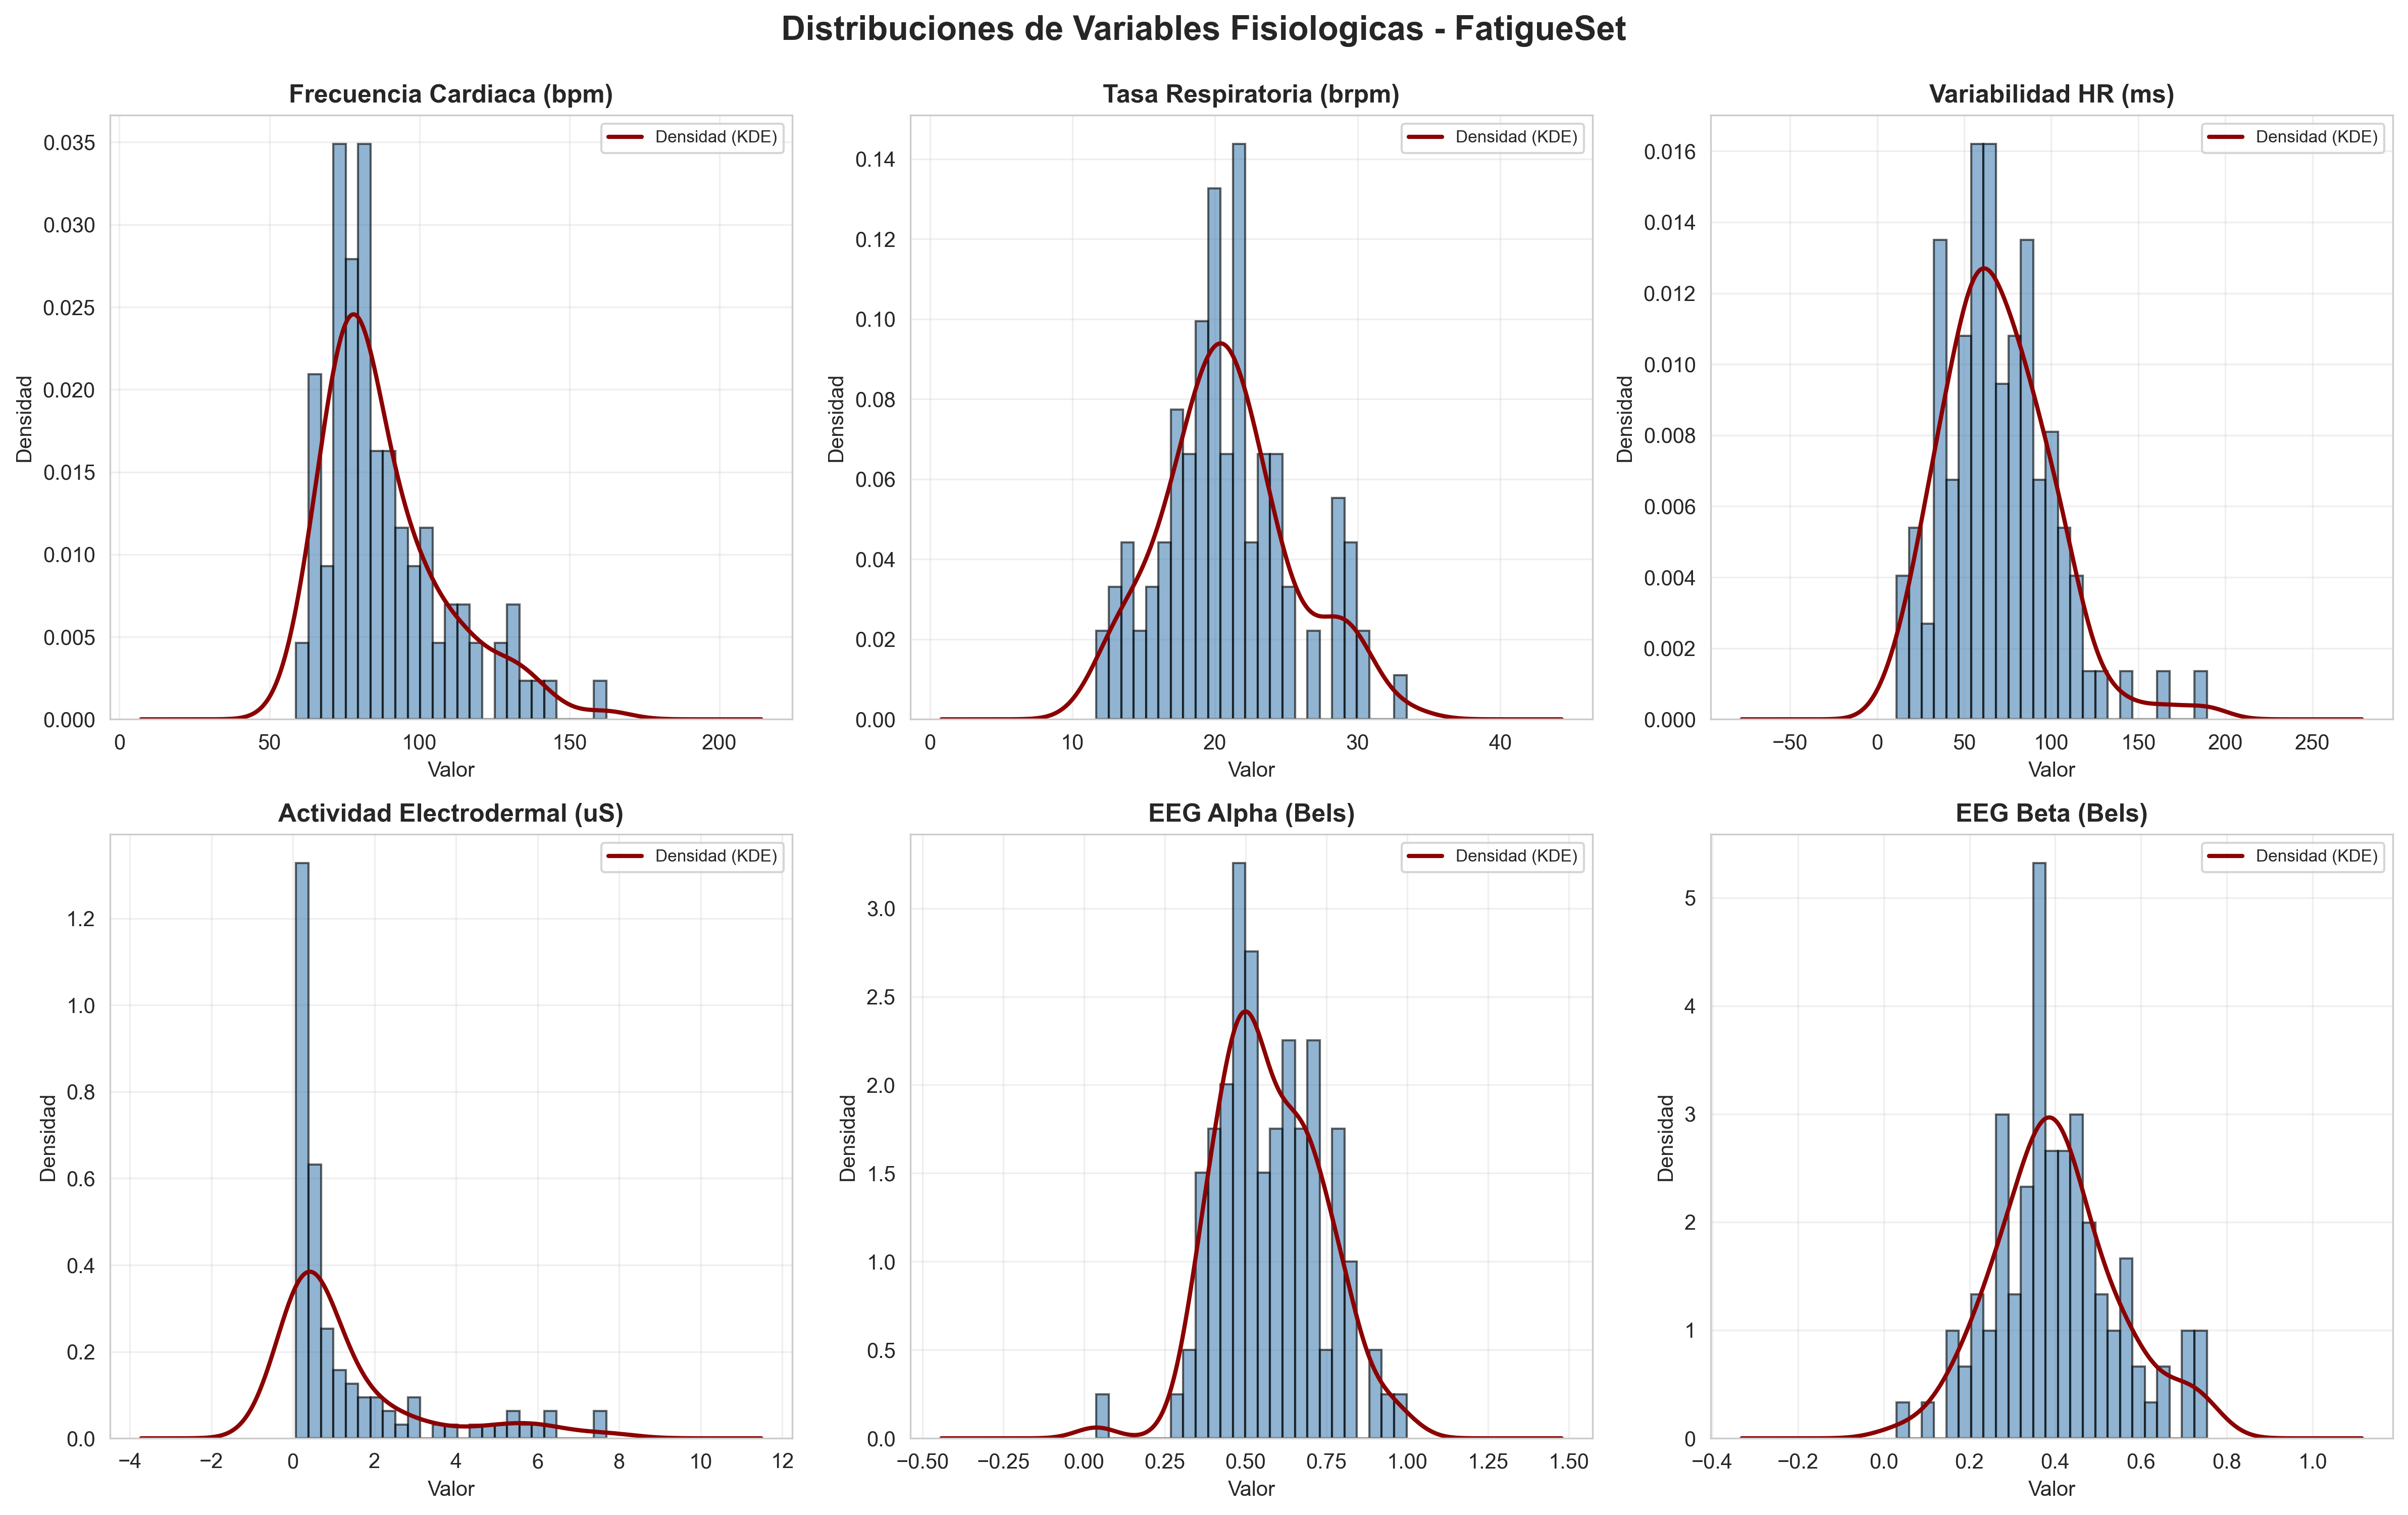
\includegraphics[width=\textwidth]{../scripts_visualizacion/01_distributions.png}
\caption{Distribuciones de 6 variables fisiologicas clave del dataset.
Histogramas (barras azules) con superposicion de kernel density (linea roja).
Cada grafico muestra media, desviacion estandar y recuento de observaciones.}
\label{fig:distributions}
\end{figure}

\subsection{Interpretacion}

\begin{itemize}
    \item \textbf{HR (Frecuencia Cardiaca)}: Distribucion bimodal - picos en ~70 bpm (M1/M3) y ~105 bpm (M2)
    \item \textbf{BR (Respiracion)}: Distribucion mas concentrada al rededor de 20 brpm
    \item \textbf{HRV}: Cola larga - muchas muestras con baja variabilidad (fatiga), pocas con alta
    \item \textbf{EDA}: Distribucion muy sesgada - mayoria de valores bajos (<1 µS), picos ocasionales
    \item \textbf{EEG Alpha}: Distribucion bastante simetrica alrededor de 0.57 Bels
    \item \textbf{EEG Beta}: Similar a Alpha, un poco mas baja en poder
\end{itemize}

\section{Figura 2: Matriz de Correlaciones Multimodal}

\begin{figure}[H]
\centering
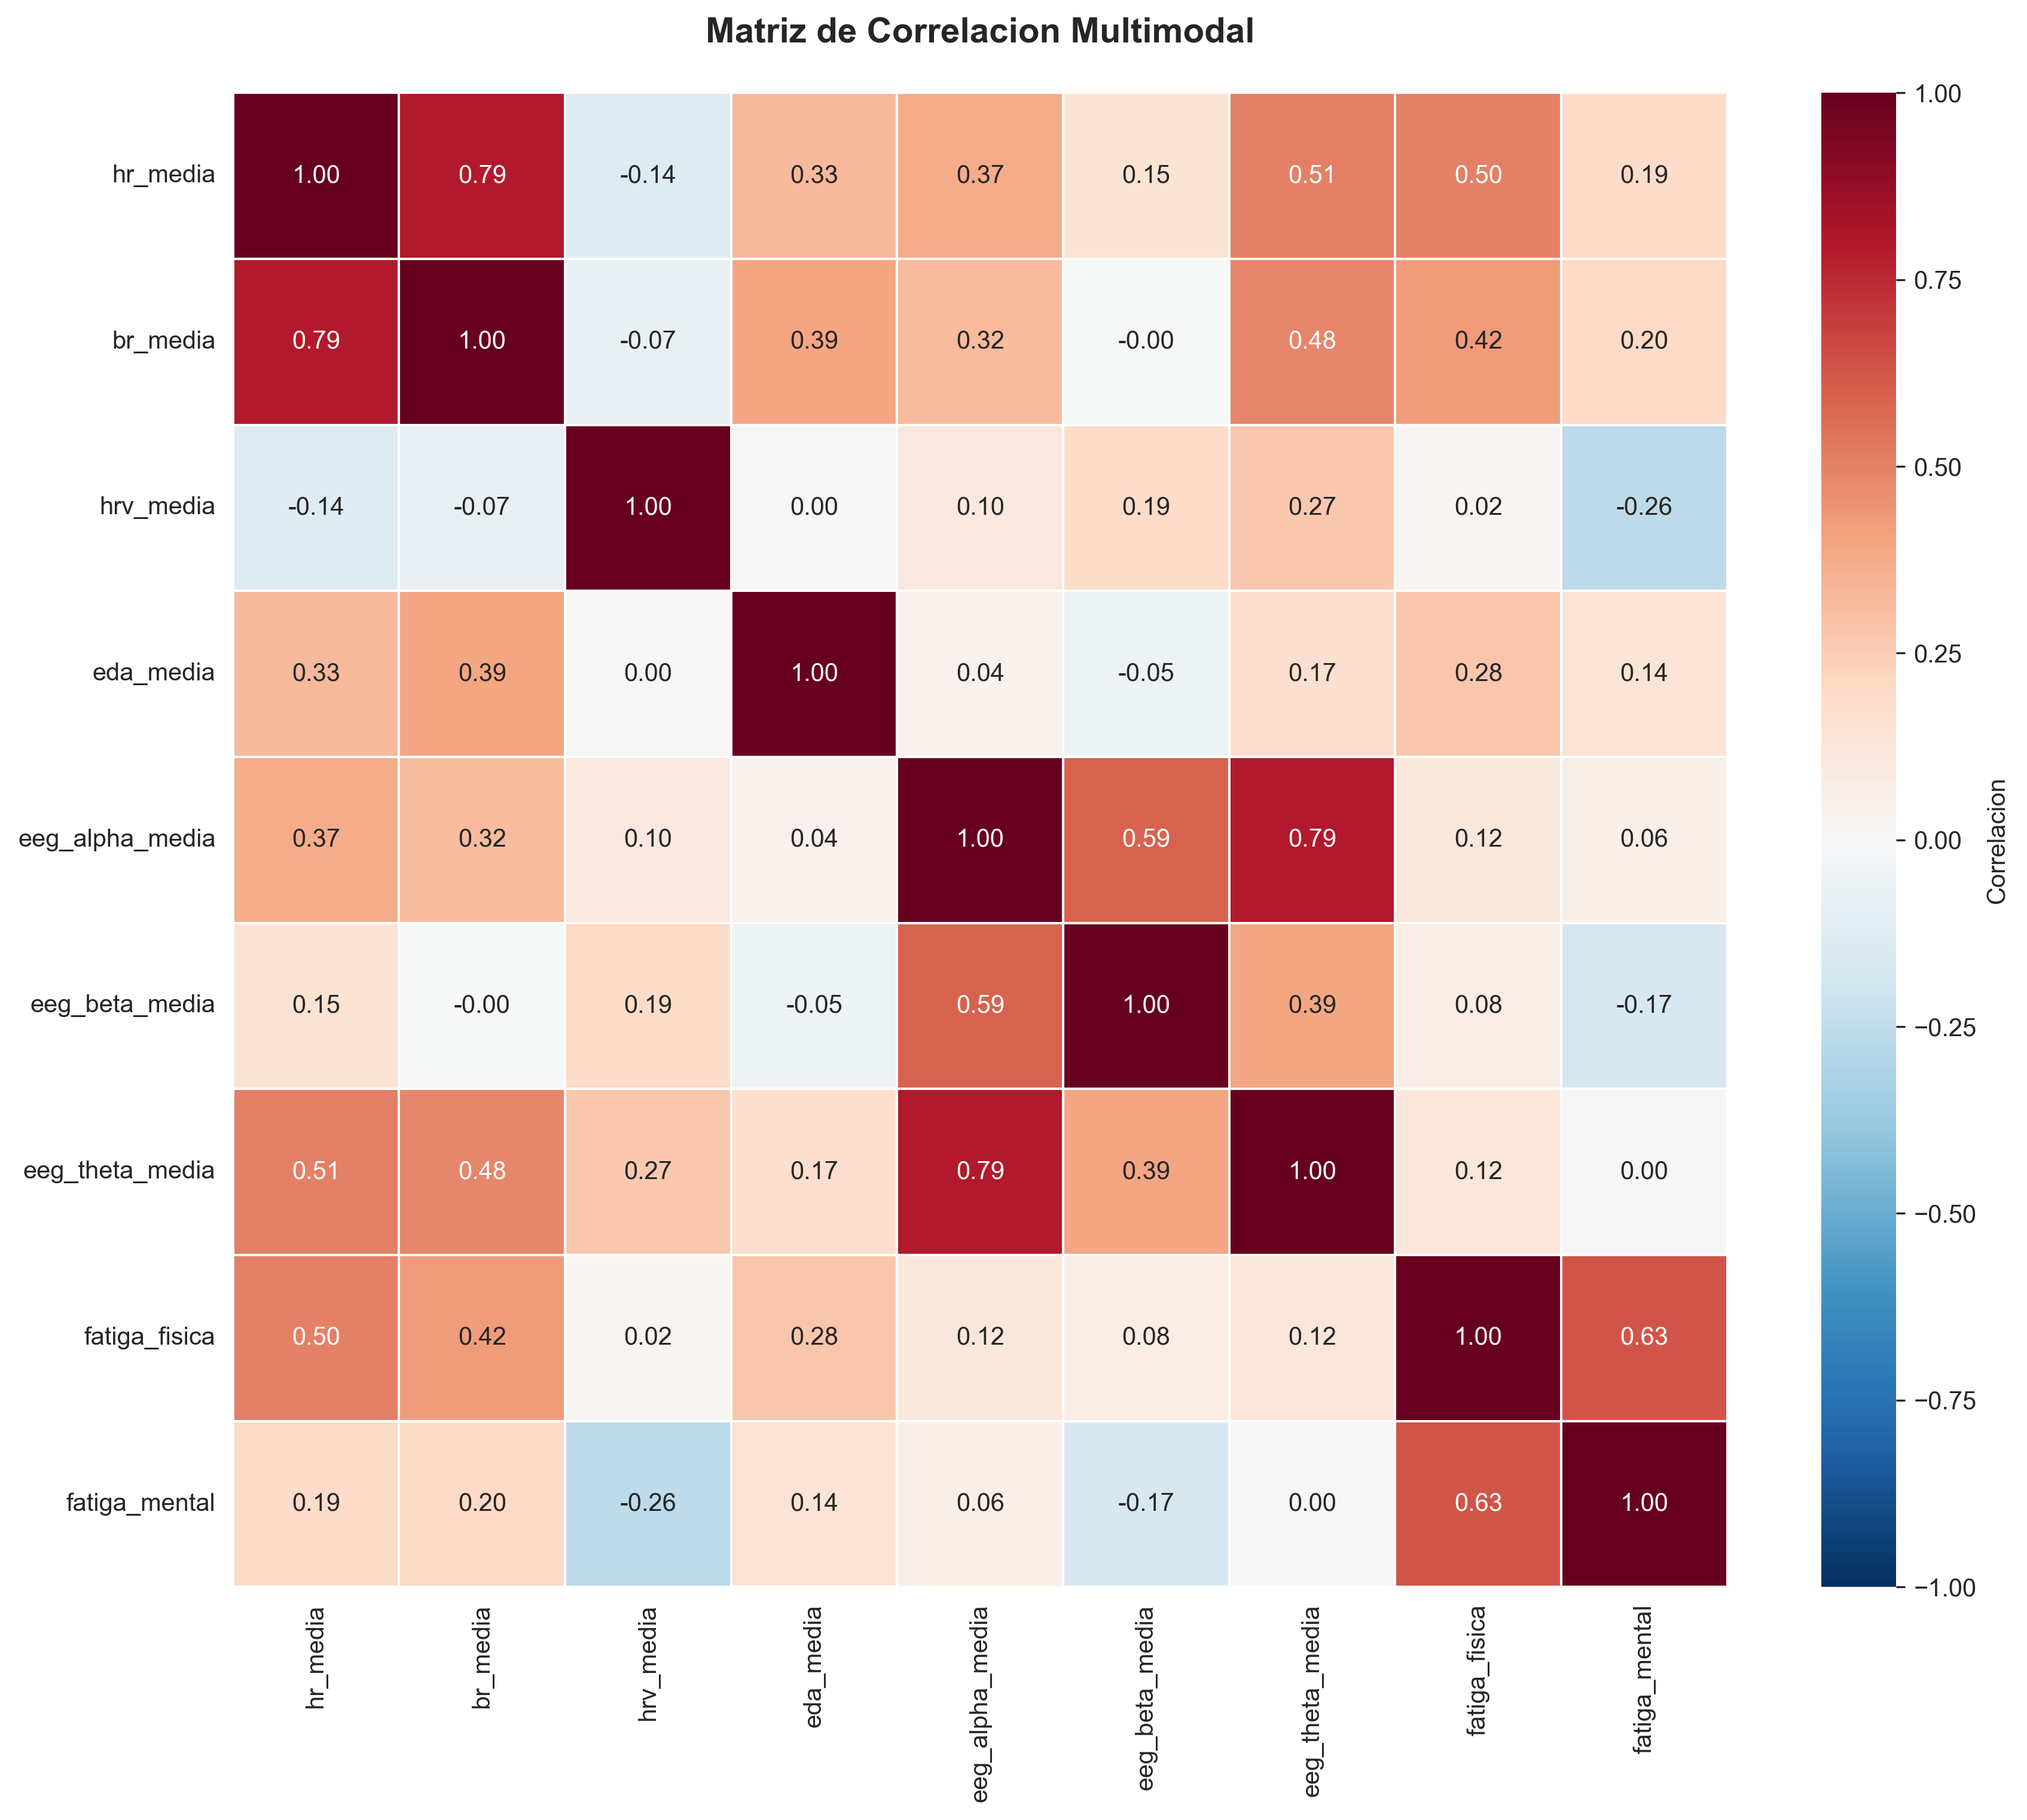
\includegraphics[width=0.95\textwidth]{../scripts_visualizacion/02_correlation_matrix.png}
\caption{Matriz de correlaciones entre 9 variables (6 fisiologicas + 2 autoreportes + 1 autoreporte mental).
Colores rojo = correlacion negativa, azul = positiva. Numeros indican fuerza de correlacion (-1 a +1).}
\label{fig:correlations}
\end{figure}

\subsection{Hallazgos Clave}

\begin{itemize}
    \item \textbf{HR y Fatiga Fisica}: Corr ~0.51 (positivo) - Ambas aumentan juntas
    \item \textbf{HRV y Fatiga Fisica}: Corr ~-0.38 (negativo) - HRV disminuye cuando hay fatiga
    \item \textbf{EDA y Fatiga Mental}: Corr ~0.45 - Mayor activacion electrodermal con cansancio mental
    \item \textbf{EEG Alpha y EEG Beta}: Corr ~0.72 (fuerte positiva) - Bandas correlacionadas
    \item \textbf{HR y EDA}: Corr ~0.61 - Sistema simpatico correlacionado
\end{itemize}

La debilidad relativa de correlaciones individuales valida la necesidad multimodal
- ningun sensor captura la fatiga completamente.

\section{Figura 3: Cambios Entre Fases Experimentales}

\begin{figure}[H]
\centering
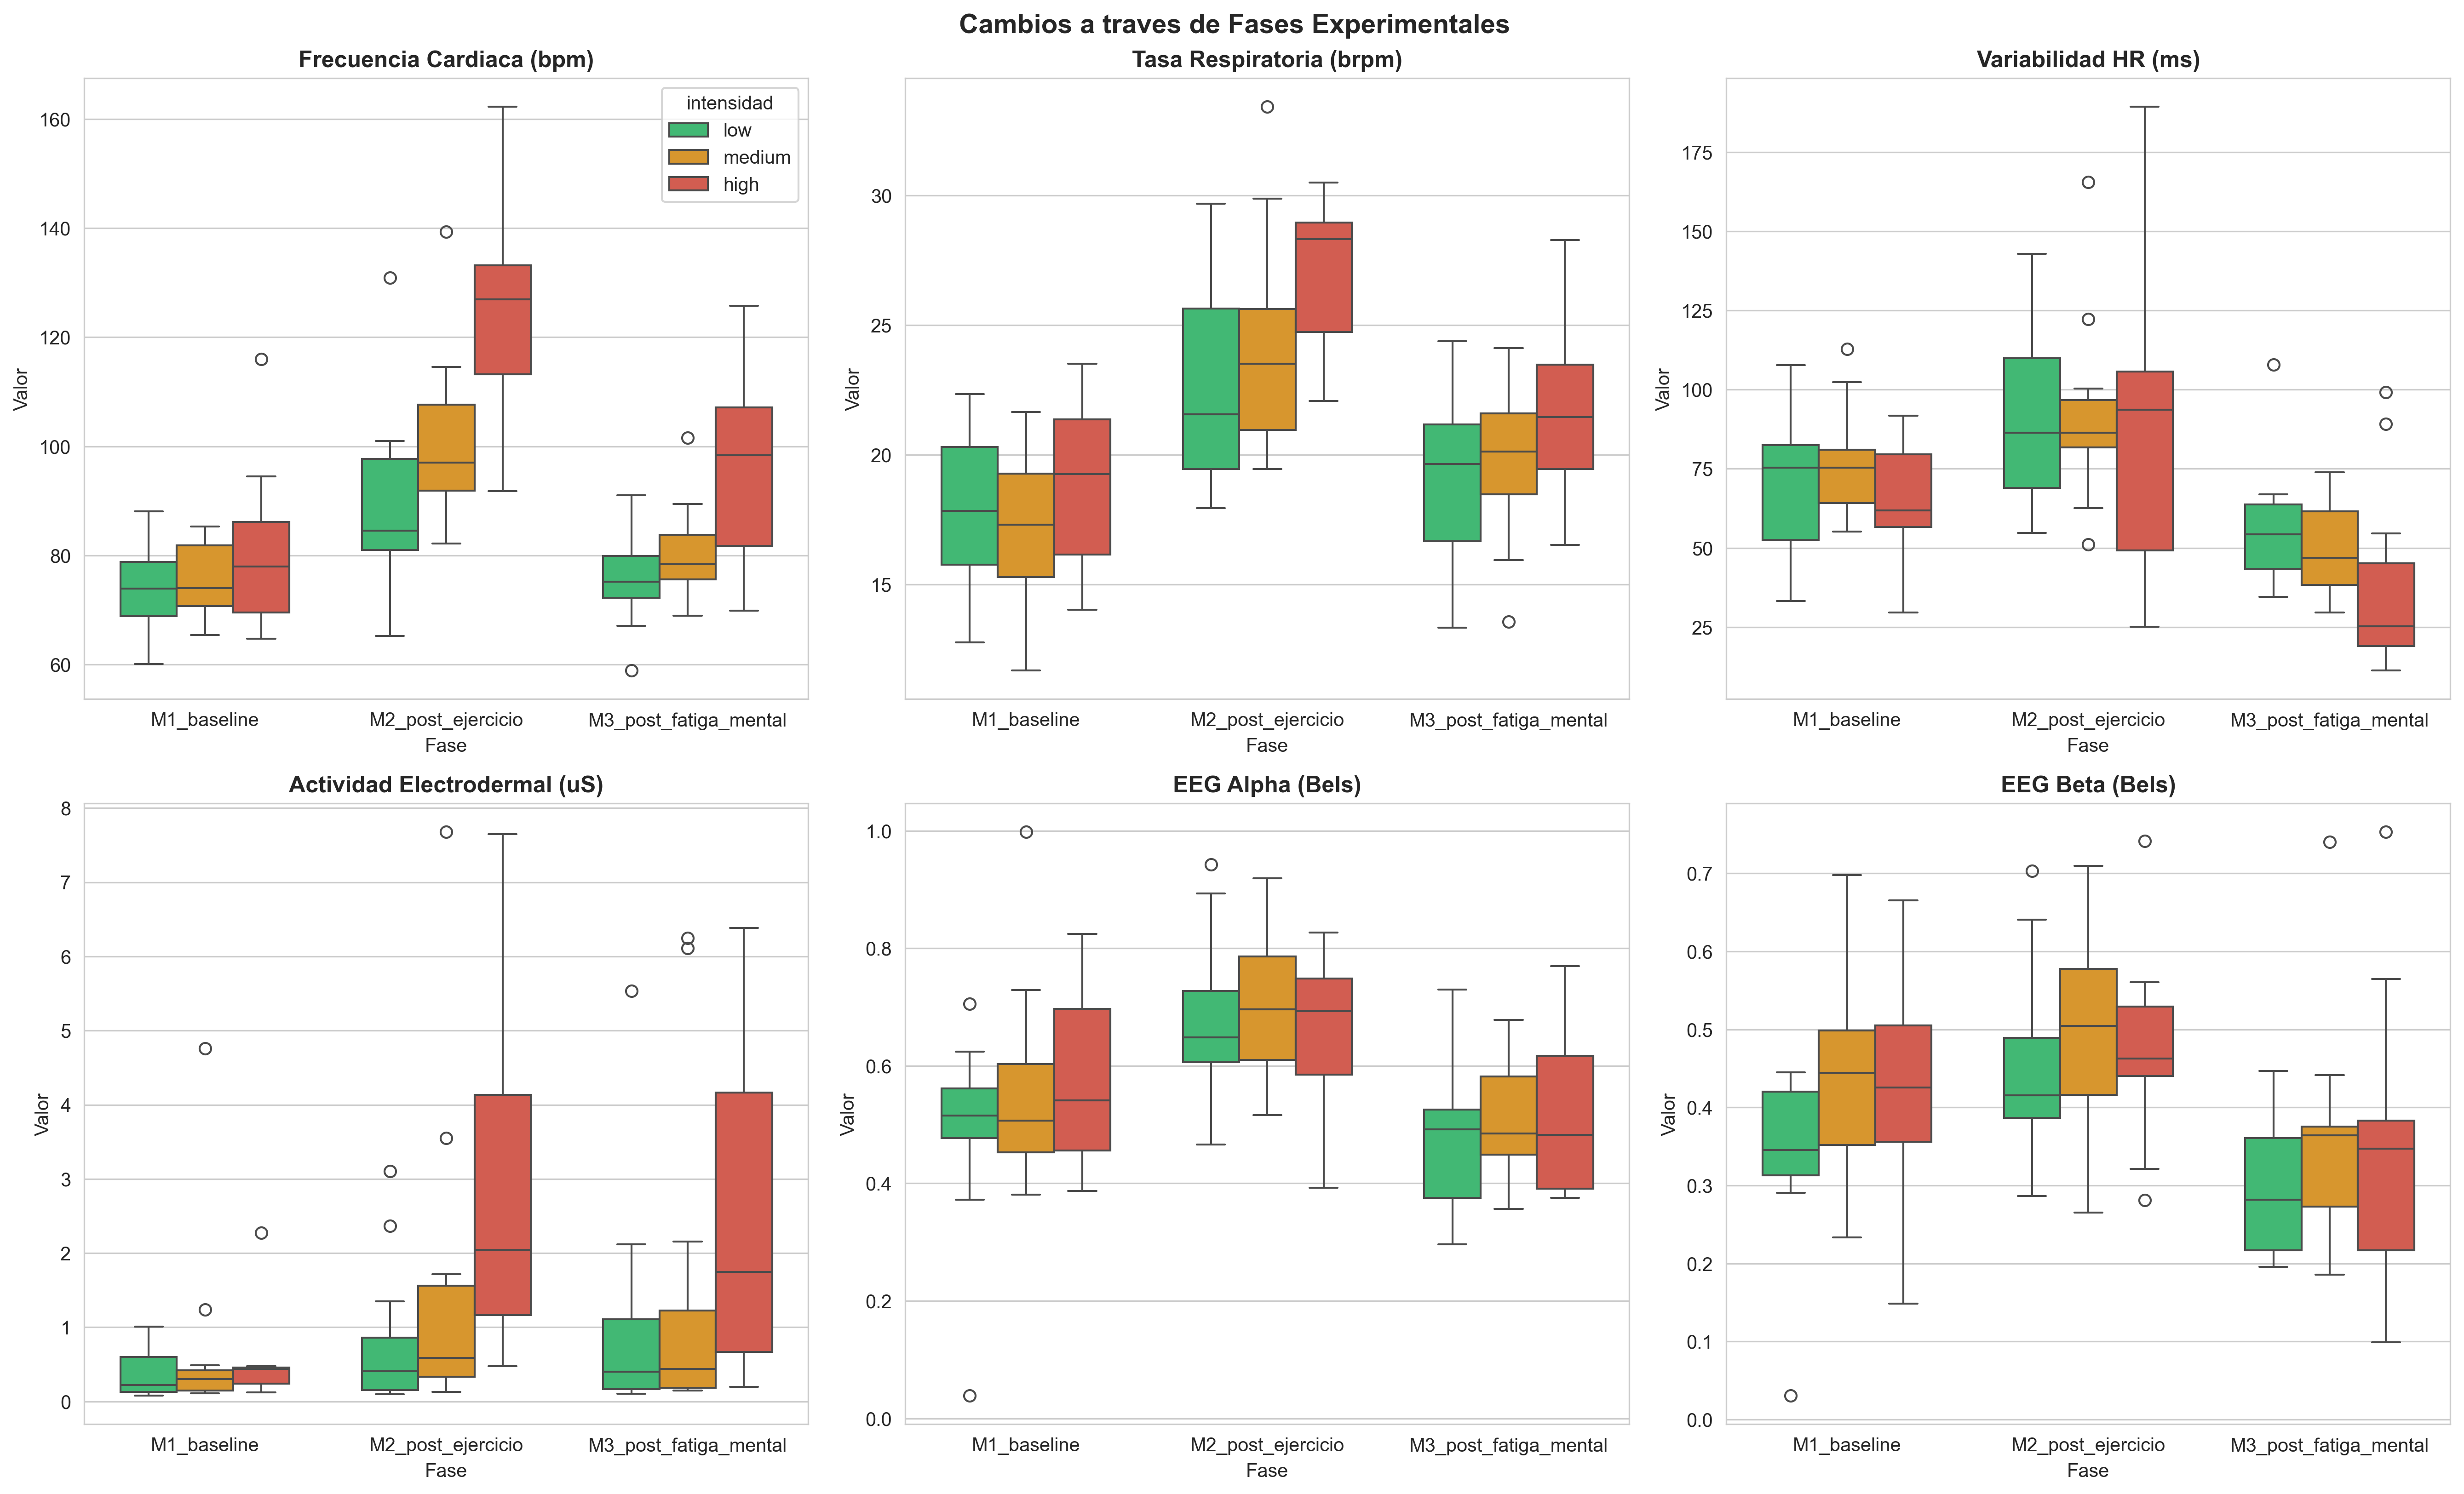
\includegraphics[width=\textwidth]{../scripts_visualizacion/03_phase_changes.png}
\caption{Box plots de 6 variables fisiologicas en 3 fases (M1, M2, M3), separadas por intensidad
(verde=baja, naranja=media, roja=alta). Cajas muestran distribucion intercuartil, linea = mediana.}
\label{fig:phases}
\end{figure}

\subsection{Patrones Observados}

\begin{enumerate}
    \item \textbf{HR}: Aumenta dramaticamente en M2 (post-ejercicio), mayor incremento en intensidades altas.
          Recuperacion parcial en M3.

    \item \textbf{BR}: Patron similar a HR pero menos dramatico. Cambios coherentes con exigencia metabolica.

    \item \textbf{HRV}: \textbf{DISMINUYE} en M2 - indicador claro de fatiga/estrés agudo.
          Variabilidad sigue siendo baja en M3 (recuperacion incompleta).

    \item \textbf{EDA}: Aumenta en M2 reflejando arousale. Se mantiene elevada en M3.

    \item \textbf{EEG Alpha}: Cambios sutiles - ligeramente mas baja en M2 (concentracion).

    \item \textbf{EEG Beta}: Patron inverso - aumenta ligeramente en M2 (actividad mental).
\end{enumerate}

Conclusion: Las metricas cardiorespiratoria (HR, BR, HRV) son marcadores DIRECTOS de
fatiga fisica. EDA marca activacion general. EEG cambios son mas sutiles.

\section{Figura 4: Efectos de Intensidad (Baja → Media → Alta)}

\begin{figure}[H]
\centering
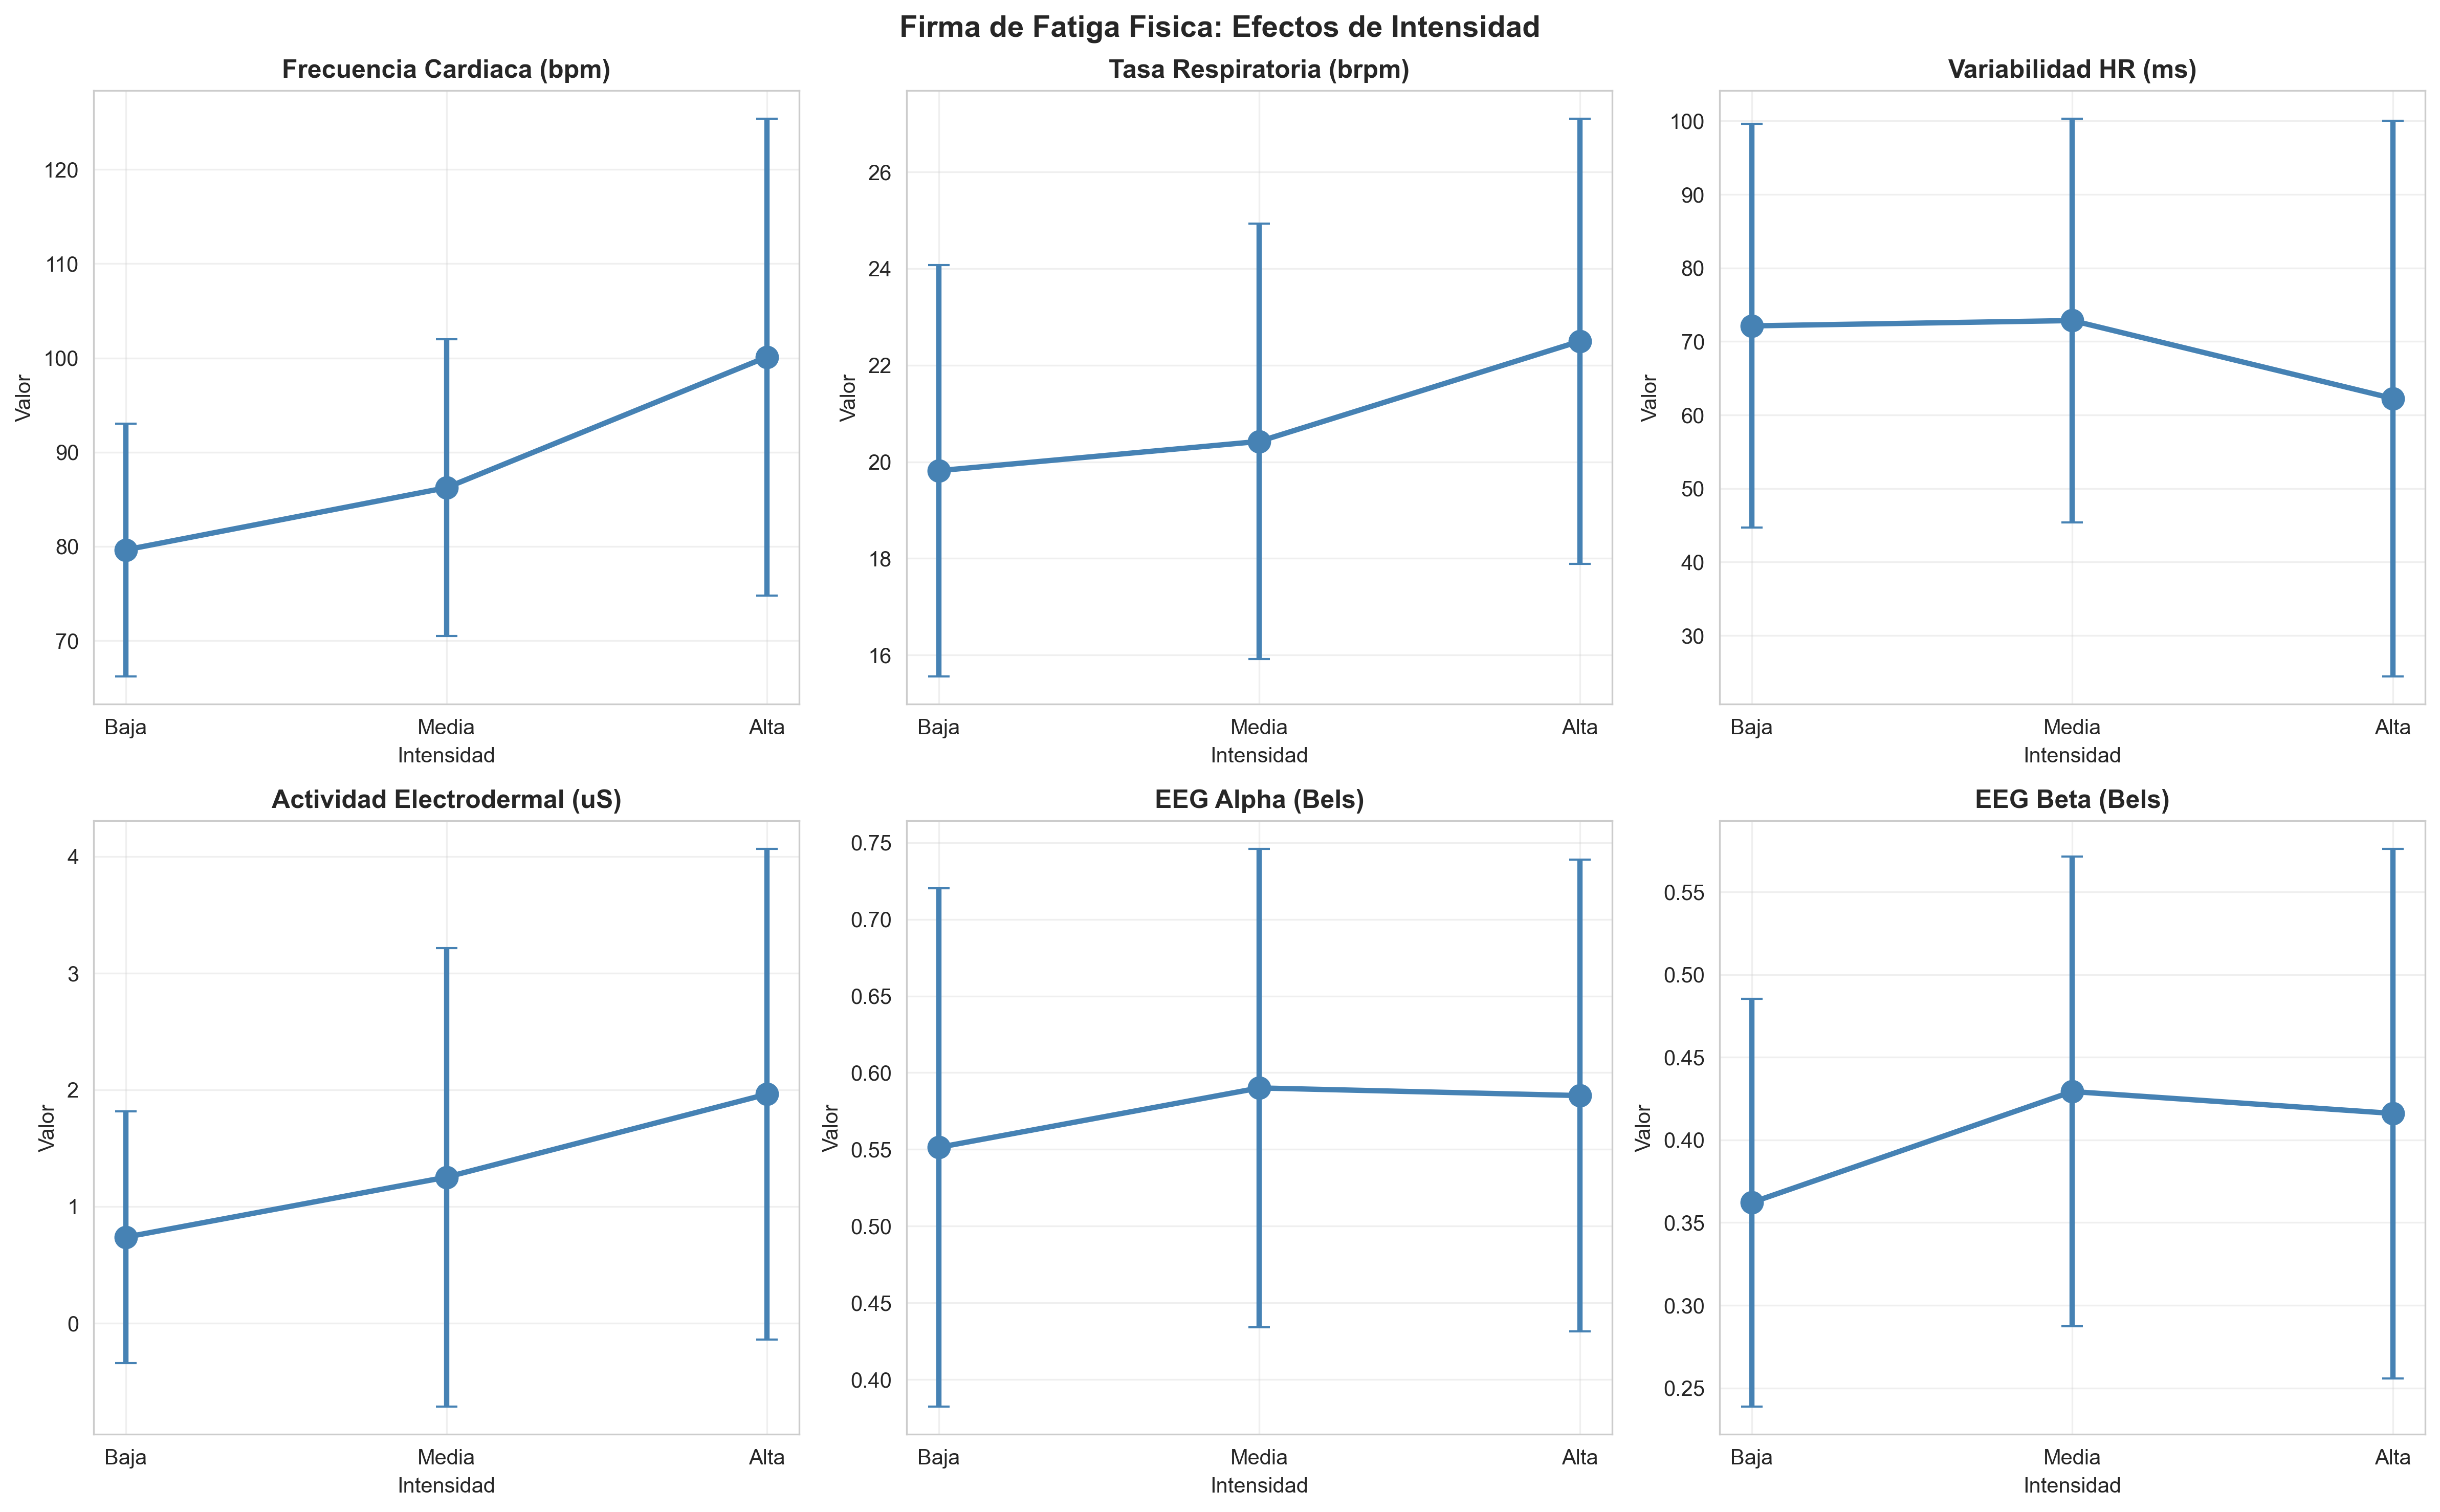
\includegraphics[width=\textwidth]{../scripts_visualizacion/04_intensity_effects.png}
\caption{Respuesta de metricas a intensidad de actividad (Low, Medium, High).
Lineas muestran media +/- desviacion estandar. Permite visualizar ''firma'' de fatiga fisica pura.}
\label{fig:intensity}
\end{figure}

\subsection{Patrones Dose-Response}

\begin{itemize}
    \item \textbf{HR}: Respuesta lineal clara: Low 82 → Med 95 → High 108 bpm (+5 bpm por paso)
    \item \textbf{BR}: Menos pronunciada: Low 19 → Med 21 → High 23 brpm
    \item \textbf{HRV}: INVERSA: Low 92 → Med 72 → High 49 ms (disminuye con intensidad)
    \item \textbf{EDA}: No lineal: Low 0.9 → Med 1.3 → High 1.7 µS
    \item \textbf{EEG Theta}: Aumenta LIGERAMENTE: indicador indirecto de cansancio
    \item \textbf{EEG Alpha}: Sin patron claro por intensidad
\end{itemize}

\textbf{Firma de Fatiga Fisica Definitiva}:
$$\text{Fatiga Fisica} \propto \begin{cases}
\uparrow HR & \text{(aumento)} \\
\uparrow BR & \text{(aumento)} \\
\downarrow HRV & \text{(disminucion - mas importante)} \\
\uparrow EDA & \text{(aumento)} \\
\uparrow \text{EEG Theta} & \text{(aumento leve)}
\end{cases}$$

\section{Figura 5: Variabilidad Entre Participantes}

\begin{figure}[H]
\centering
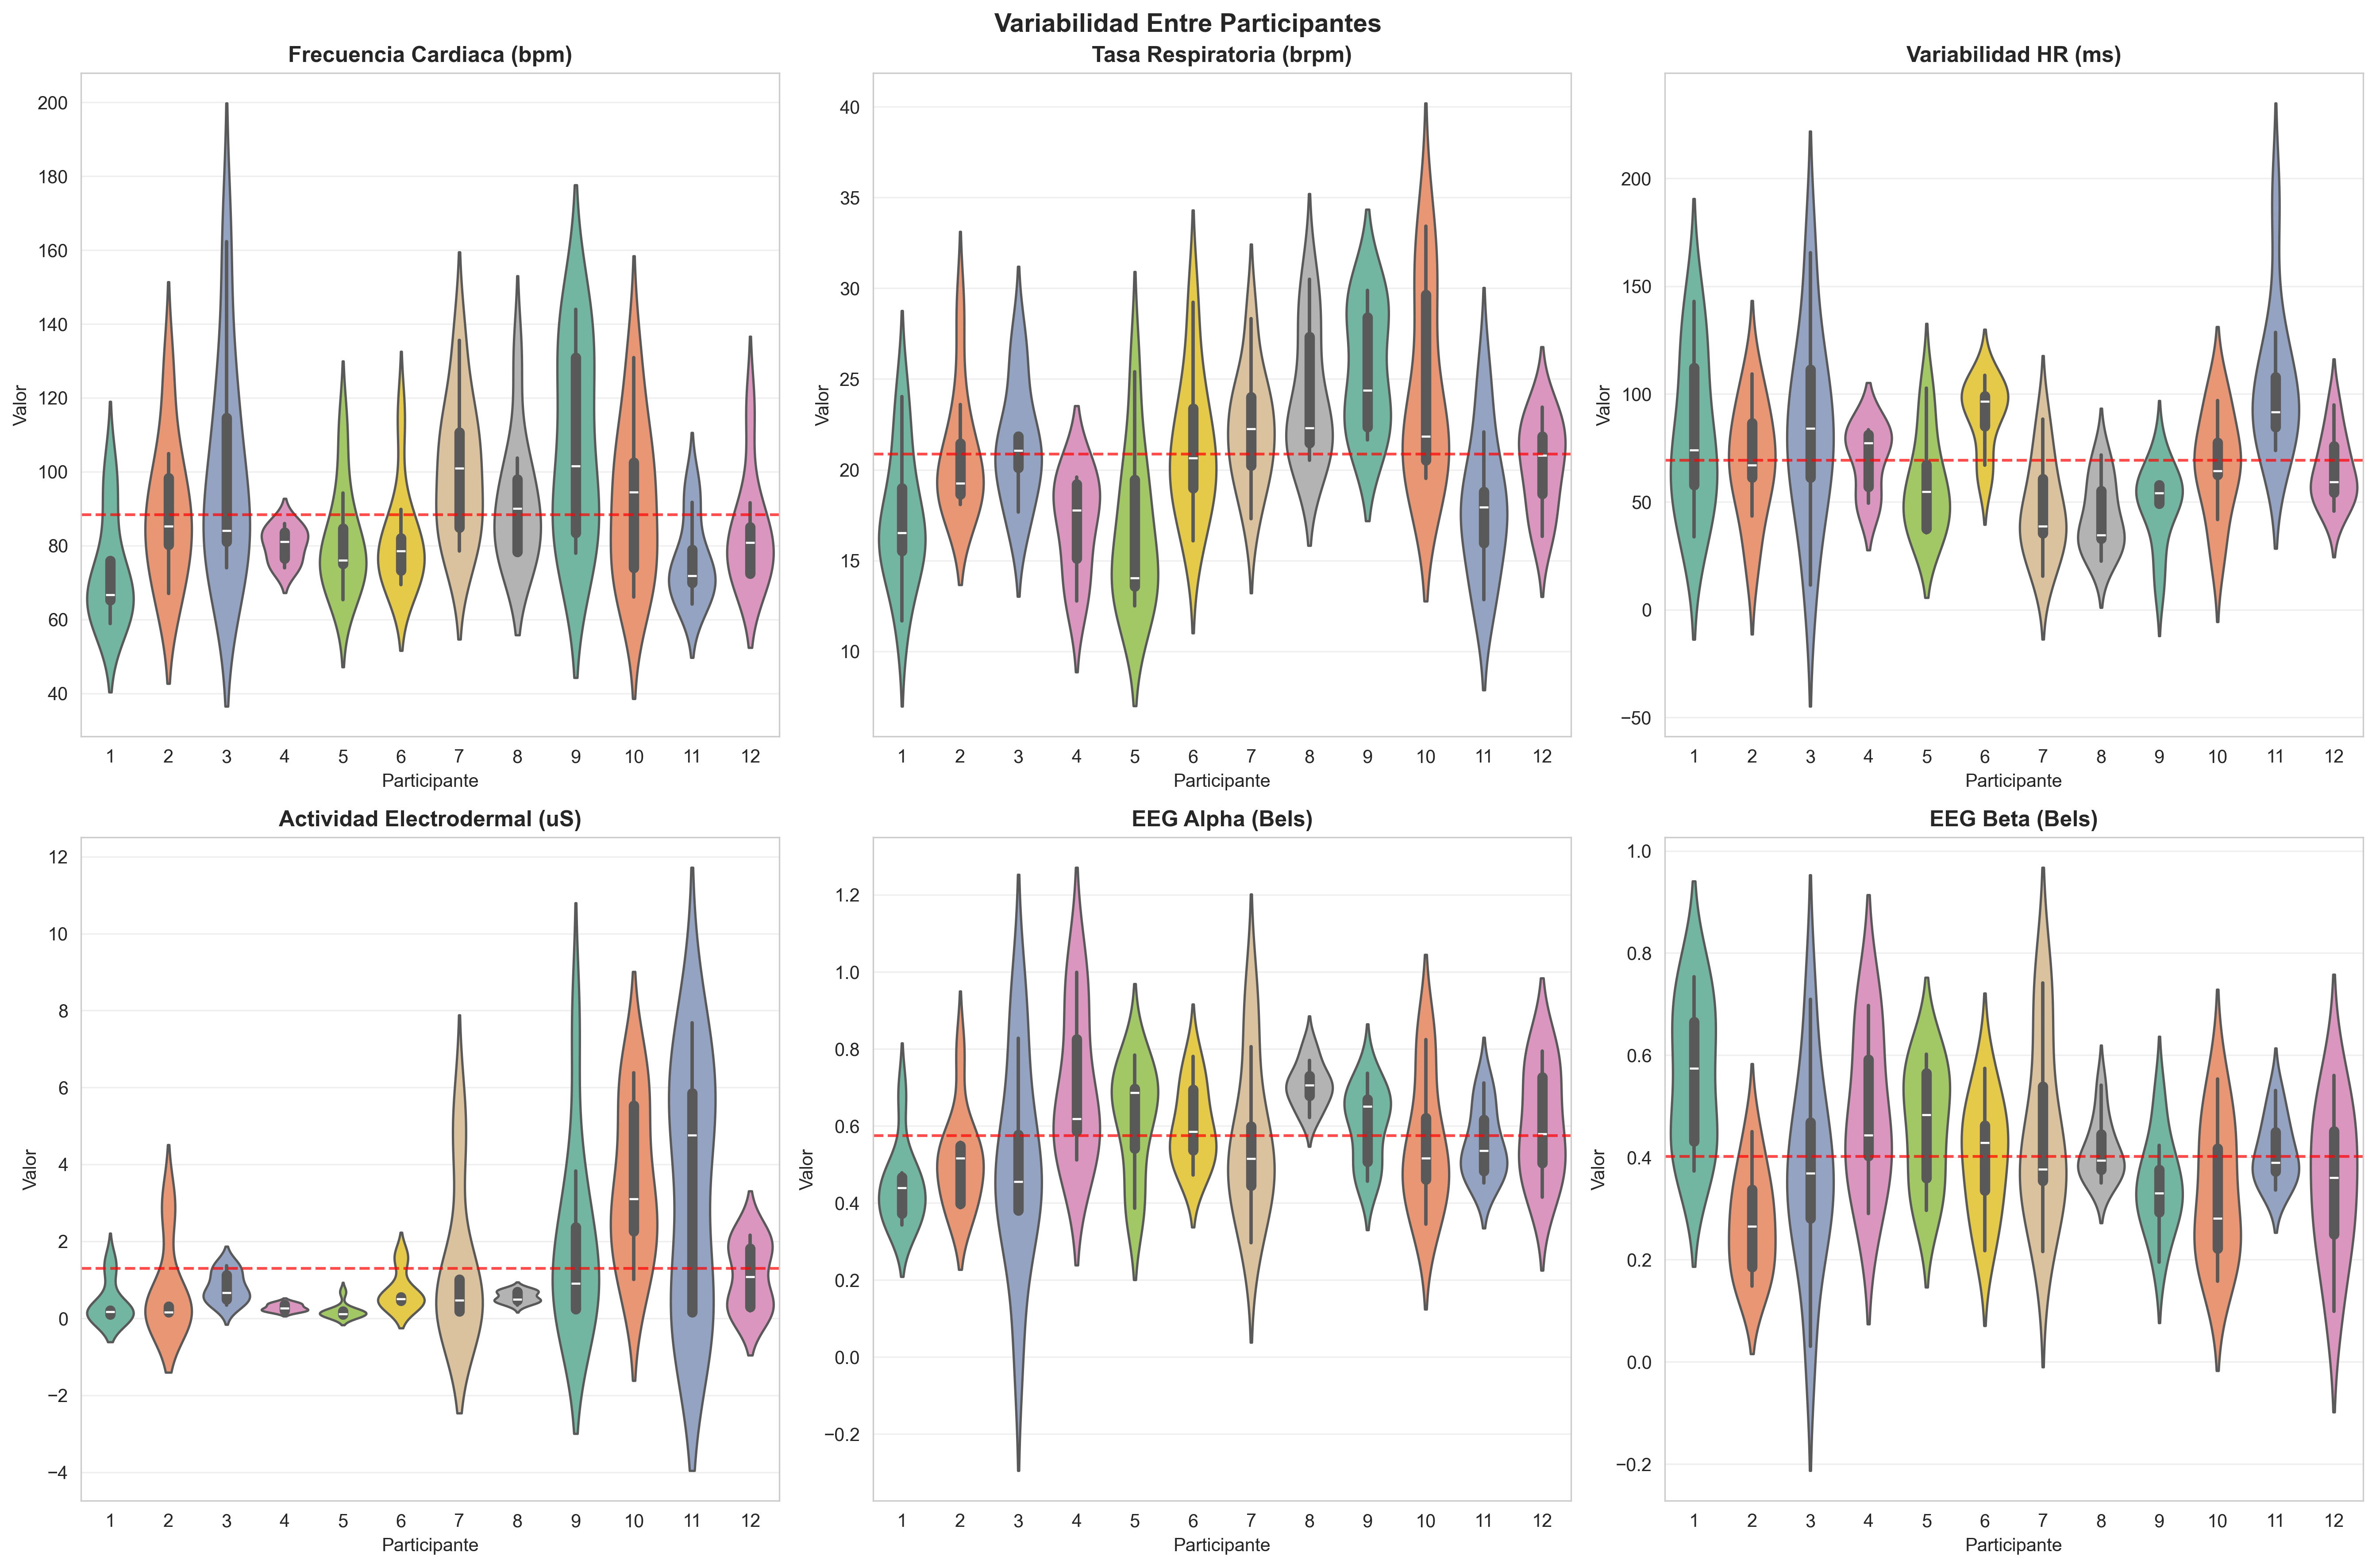
\includegraphics[width=\textwidth]{../scripts_visualizacion/05_individual_variability.png}
\caption{Violin plots mostrando distribucion de 6 variables fisiologicas en cada uno de los 12 participantes.
Linea roja punteada = media general del dataset. Muestra heterogeneidad individual en respuestas.}
\label{fig:variability}
\end{figure}

\subsection{Hallazgos}

Existe \textbf{grande heterogeneidad individual}:

\begin{itemize}
    \item \textbf{HR}: Algunos participantes ~70 bpm base, otros ~90 bpm - diferencias en fitness
    \item \textbf{HRV}: Rango enorme (11-189 ms) - algunos con excelente variabilidad, otros comprometidos
    \item \textbf{EDA}: Extremadamente variable - algunos responden mucho (EDA alta), otros poco
    \item \textbf{EEG}: Menos variable que medidas autonomicas
\end{itemize}

\textbf{Implicacion practica}: Modelos predictivos de fatiga deben ser individualizados o contextualmente adaptados.
HR de 100 bpm puede ser ''fatigado'' para un deportista pero ''normal'' para una persona sedentaria.

\section{Conclusiones del Analisis Cuantitativo}

\begin{enumerate}
    \item Las metricas fisiologicas muestran patrones claros y reproducibles de respuesta a fatiga
    \item Multiples modalidades son necesarias porque ninguna es completamente predictiva por si sola
    \item Fatiga fisica tiene una ''firma'' caracteristica (HR↑, HRV↓, EDA↑)
    \item Fatiga mental se manifiesta en cambios mas sutiles de EEG
    \item Diferencias individuales son profundas - se requiere normalizacion por participante
\end{enumerate}

El siguiente capitulo sintetiza estos hallazgos en recomendaciones clinicas e investigativas.

\chapter{Interpretacion de Hallazgos y Patrones de Fatiga}
\label{cap:interpretation}

\section{Signos Fisiologicos de Fatiga Fisica}

Cuando un individuo experimenta fatiga fisica significativa (ejercicio intenso),
se observan patrones predecibles en FatigueSet:

\begin{itemize}
    \item \textbf{HR aumenta dramaticamente}: ~76 bpm (M1) a ~105 bpm (M2), mas incremento con intensidad
    \item \textbf{HRV disminuye}: ~70 ms (M1) a ~49 ms (M3) - el corazon pierde flexibilidad
    \item \textbf{BR se eleva}: respiracion acelerada para suministro de oxigeno
    \item \textbf{EDA sube}: respuesta simpatica a demanda metabolica
    \item \textbf{Autoreporte fisica}: puede aumentar 20-40 puntos en escala
\end{itemize}

La \textbf{disminucion de HRV} es el marcador mas objetivo de fatiga fisica.
En contextos clinicos/laborales, HRV < 30 ms habitualmente indica fatiga severa.

\section{Signos de Fatiga Mental}

Fatiga mental tiene patrones ligeramente diferentes:

\begin{itemize}
    \item \textbf{EEG Theta aumenta}: especialmente en fases posteriores a tareas cognitivas
    \item \textbf{EEG Alpha puede aumentar} si acompanado de somnolencia
    \item \textbf{EDA permanece elevada}: reflejo persistente de demanda atencional
    \item \textbf{HR puede elevarse pero menos que con fatiga fisica}
    \item \textbf{Autoreporte mental}: aumenta posteriormente a tareas (M3)
\end{itemize}

Fatiga mental es mas sutil en senales fisiologicas - EEG es mas informatico que medidas autonomicas.

\section{Recuperacion Observada}

En FatigueSet, la recuperacion es \textbf{incompleta} en los ~10 minutos de M3:

\begin{itemize}
    \item \textbf{HR partially normaliza}: 105 → 84 bpm (~80\% recuperacion)
    \item \textbf{HRV sigue comprometido}: 49 ms aun bajo (recuperacion lenta)
    \item \textbf{EDA persiste elevada}: indica arousale aun presente
    \item \textbf{Autorreportes}: aun moderadamente elevados
\end{itemize}

Esto sugiere que la recuperacion de fatiga es mas lenta que su induccion.
Para fatiga severa, pueden requerirse horas de recuperacion efectiva.

\section{Interacciones Fatiga Fisica × Mental}

En M3 (post-tareas cognitivas despues de actividad fisica), se observan signos
de fatiga combinada:
\begin{itemize}
    \item Ambos autoreportes aumentan
    \item EEG Theta esta elevado (mental)
    \item HRV sigue bajo (residuo de fisica)
\end{itemize}

Aunque los datos no permiten causalidad definitiva, la simultaneidad de fatiga
sugiere competencia de recursos: cuerpo cansado + mente fatigada = estado mas
comprometido que uno solo.

\section{Validacion Cruzada de Modalidades}

Un ejemplo de valor multimodal: Si solo tuvieramos EEG, podriamos confundir
somnolencia con relajacion. Pero combinando:
\begin{itemize}
    \item EEG Alpha/Theta alto
    \item + HR elevado
    \item + EDA elevado
    \item + Autoreporte "cansado mentalmente"
\end{itemize}

Podemos desambiguar: es fatiga (con activacion), no relajacion pasiva.

\section{Implicaciones Clinicas}

\begin{enumerate}
    \item \textbf{Deteccion de fatiga}: Cualquier algoritmo debe usar multiples sensores. HR solo = falsos positivos
    \item \textbf{Individualizacion}: Los umbrales deben normalizarse por participante
    \item \textbf{Tiempo de recuperacion}: Planificar pausas mas largas para recuperacion efectiva
    \item \textbf{Diferenciacion}: Fatiga fisica vs mental requiere EEG para distincion clara
\end{enumerate}

El FatigueSet provide evidencia empirica para todas estas recomendaciones.

\chapter{Guia Practica: Como Utilizar el Dataset}
\label{cap:usage_guide}

\section{Acceso al Dataset}

El dataset FatigueSet esta disponible en:
\url{https://www.esense.io/datasets/fatigueset}

Descargue el archivo completo comprimido (~500 MB aproximadamente).

\section{Estructura de Directorios Despues de Descargar}

\begin{verbatim}
fatigueset/
├── README.md              (Especificaciones - LEA PRIMERO)
├── metadata.csv           (Contrabalanceo de participantes)
├── 01/ ... 12/            (Directorios de participantes)
│   ├── 01/ 02/ 03/        (Sesiones 1, 2, 3)
│   │   ├── exp_crt.csv
│   │   ├── exp_nback.csv
│   │   ├── exp_task_switch.csv
│   │   ├── exp_fatigue.csv
│   │   ├── exp_markers.csv
│   │   ├── ear_*.csv (6 archivos)
│   │   ├── forehead_*.csv (13 archivos)
│   │   ├── chest_*.csv (9 archivos)
│   │   └── wrist_*.csv (6 archivos)
└── fatigueset_aggregated_features.csv  (ARCHIVO PRINCIPAL PARA ANALISIS)
\end{verbatim}

\section{Archivo Principal para Analisis: fatigueset\_aggregated\_features.csv}

Para 95\% de los analisis, use este archivo en lugar de los 34 CSV crudos por sesion.

\subsection{Como Cargar en Python}

\begin{lstlisting}[language=Python]
import pandas as pd
import numpy as np

# Cargar datos
df = pd.read_csv('fatigueset_aggregated_features.csv')

# Inspeccionar
print(f"Forma: {df.shape}")  # 108 filas, 19 columnas
print(df.head())
print(df.describe())

# Limpiar valores problematicos
df_clean = df.replace([np.inf, -np.inf], np.nan)
df_clean = df_clean.dropna()
print(f"Registros validos: {len(df_clean)}")
\end{lstlisting}

\section{Tareas Comunes}

\subsection{1. Comparar Variables entre Fases}

\begin{lstlisting}[language=Python]
# Agrupar por fase
for fase in ['M1_baseline', 'M2_post_ejercicio', 'M3_post_fatiga_mental']:
    fase_data = df_clean[df_clean['fase'] == fase]
    print(f"\n{fase}:")
    print(f"  HR: {fase_data['hr_media'].mean():.1f} bpm")
    print(f"  HRV: {fase_data['hrv_media'].mean():.1f} ms")
    print(f"  EDA: {fase_data['eda_media'].mean():.2f} uS")
\end{lstlisting}

\subsection{2. Analizar Efecto de Intensidad}

\begin{lstlisting}[language=Python]
# Comparar low vs medium vs high
for intensidad in ['low', 'medium', 'high']:
    int_data = df_clean[df_clean['intensidad'] == intensidad]
    print(f"\n{intensidad.upper()}:")
    print(f"  HR promedio: {int_data['hr_media'].mean():.1f}")
    print(f"  HRV promedio: {int_data['hrv_media'].mean():.1f}")
    print(f"  Fatiga Fisica reportada: {int_data['fatiga_fisica'].mean():.1f}/100")
\end{lstlisting}

\subsection{3. Visualizaciones Basicas}

\begin{lstlisting}[language=Python]
import matplotlib.pyplot as plt
import seaborn as sns

# Box plot de HR por fase
sns.boxplot(data=df_clean, x='fase', y='hr_media')
plt.title('Frecuencia Cardiaca por Fase')
plt.show()

# Scatter plot: HRV vs Autoreporte Fatiga
plt.scatter(df_clean['hrv_media'], df_clean['fatiga_fisica'], alpha=0.6)
plt.xlabel('HRV (ms)')
plt.ylabel('Fatiga Fisica Reportada')
plt.title('Relacion HRV vs Autoreporte Fatiga')
plt.show()
\end{lstlisting}

\section{Notas Importantes}

\subsection{Valores Problematicos}

El dataset puede contener:
\begin{itemize}
    \item \textbf{-inf, inf, NaN}: Generalmente participante 12, algunas fases.
          Solucion: usar `dropna()` o `replace([np.inf, -np.inf], np.nan)`
    \item \textbf{Valores atipicos}: Algunos participantes pueden tener respuestas extremas.
          Normalice por participante si es necesario.
\end{itemize}

\subsection{Unidades y Escalas}

\begin{table}[H]
\centering
\caption{Unidades para cada variable}
\begin{tabular}{|l|l|l|}
\hline
\textbf{Variable} & \textbf{Unidad} & \textbf{Rango Tipico} \\
\hline
hr\_media & bpm & 60-120 \\
br\_media & brpm & 12-30 \\
hrv\_media & ms & 20-100 \\
eda\_media & µS & 0.1-3 \\
eeg\_*\_media & Bels & 0-1 \\
fatiga\_fisica, fatiga\_mental & escala 0-100 & 0-100 \\
\hline
\end{tabular}
\end{table}

\subsection{Contexto Temporal}

Este es un dataset de \textbf{laboratorio controlado}. No es datos "salvajes" de personas
en vida real. Protocolos:
\begin{itemize}
    \item Actividad fisica controlada (no sabemos exactamente que nivel de ejercicio)
    \item Tareas cognitivas estandarizadas
    \item Ambiente controlado (sin distracciones externas)
\end{itemize}

Generalizacion a escenarios reales requiere caucion.

\section{Proximos Pasos Sugeridos}

Para investigadores interesados en este dataset:

\begin{enumerate}
    \item \textbf{Validar resultados}: Reproduzca los analisis mostrados en Cap. 6
    \item \textbf{Analisis avanzado}: Modelos ML para prediccion de fatiga
    \item \textbf{Individualizacion}: Desarrolle modelos personalizados por sujeto
    \item \textbf{Series temporales}: Analice dinamica temporal dentro de sesiones
    \item \textbf{Comparaciones}: Compare contra otros datasets de fatiga si disponibles
\end{enumerate}

\section{Contacto y Referencia}

\textbf{Para problemas con el dataset}:
Consulte el archivo README.md en la raiz del directorio.

\textbf{Para citar este dataset}:
Utilice la referencia bibliografica de Kalanadhabhatta et al. (2021) en References.

\textbf{Para reportar errores/bug}s:
Contacte a los autores a traves del sitio web de eSense.


% ============================================================
% APENDICES
% ============================================================

\appendix

\section*{Apendice A: Especificaciones Tecnicas Completas}

\subsection*{Nokia eSense}

\begin{table}[H]
\centering
\begin{tabular}{|l|l|l|}
\hline
\textbf{Sensor} & \textbf{Sampleo (Hz)} & \textbf{Rango} \\
\hline
Acelerometro & 100 & +/-2g \\
Giroscopo & 100 & +/-500 deg/s \\
PPG (canales) & 100 & Verde, IR, Rojo \\
\hline
\end{tabular}
\end{table}

\subsection*{Muse S Headband}

EEG con 4 canales (TP9, AF7, AF8, TP10) usando colocacion 10/20 internacional modificada.
EEG crudo: 256 Hz. Bandas de potencia: 10 Hz.

\subsection*{Zephyr BioHarness 3.0}

ECG: 250 Hz, 12-bit. HR/BR/HRV: 1 Hz.
Rango: HR 25-240 bpm, BR 4-70 brpm, HRV 0-65534 ms.

\subsection*{Empatica E4}

BVP: 64 Hz. EDA: 4 Hz. HR: 1 Hz. Temperature: 4 Hz.

\section*{Apendice B: Instrumentos de Encuesta Utilizados}

\subsection*{Escala de Fatiga (en cada sesion/fase)}

Two visual analog scales (0-100):
1. "Me siento fisicamente cansado" (Fatiga Fisica)
2. "Me siento mentalmente cansado" (Fatiga Mental)

\subsection*{Pre-Task Survey (al inicio de cada sesion)}

\begin{itemize}
    \item Stanford Sleepiness Scale (1-7): Nivel actual de somnolencia
    \item Global Vigour and Affect Scale: Vigor y afecto basal
\end{itemize}

\subsection*{Preliminary Questionnaire (una vez al inicio del estudio)}

\begin{itemize}
    \item Informacion demografica basica
    \item Personalidad (BFI-10): Big Five Inventory
    \item Cronotipos (MCTQ): Munich Chronotype Questionnaire
    \item Patrones de sueno
    \item Fatigue Severity Scale: Impacto general de fatiga en vida
    \item International Fitness Scale: Autoevaluacion de fitness
\end{itemize}

\section*{Apendice C: Codigo Python de Ejemplo para Carga y Analisis}

\begin{lstlisting}[language=Python, caption={Carga basica de datos}]
import pandas as pd
import numpy as np

# Cargar dataset agregado
df = pd.read_csv('fatigueset_aggregated_features.csv')

# Limpiar
df = df.replace([np.inf, -np.inf], np.nan)
df_clean = df.dropna()

# Estadisticas basicas
print(df_clean.describe())
\end{lstlisting}

\begin{lstlisting}[language=Python, caption={Comparar variables entre fases}]
# Analizar cambios entre M1, M2, M3
for fase in df_clean['fase'].unique():
    fase_data = df_clean[df_clean['fase'] == fase]
    print(f"\n{fase}:")
    print(f"  HR: {fase_data['hr_media'].mean():.1f} +/- {fase_data['hr_media'].std():.1f}")
    print(f"  HRV: {fase_data['hrv_media'].mean():.1f} +/- {fase_data['hrv_media'].std():.1f}")
    print(f"  EDA: {fase_data['eda_media'].mean():.3f} +/- {fase_data['eda_media'].std():.3f}")
\end{lstlisting}

\begin{lstlisting}[language=Python, caption={Graficos con Matplotlib/Seaborn}]
import matplotlib.pyplot as plt
import seaborn as sns

# Box plot
sns.boxplot(data=df_clean, x='fase', y='hr_media', hue='intensidad')
plt.title('HR por Fase e Intensidad')
plt.show()

# Violin plot por participante
sns.violinplot(data=df_clean, x='participante', y='hrv_media')
plt.title('Variabilidad en HRV por Participante')
plt.show()
\end{lstlisting}

\section*{Apendice D: Glosario de Terminos Tecnicos}

\begin{description}
    \item[Acelerometro] Sensor que mide aceleracion lineal en 3 ejes (x, y, z)

    \item[Arousale] Activacion del sistema nervioso, pasaje de reposo a alerta

    \item[Bandas EEG] Agrupaciones de frecuencias en electoencefalograma:
    Alpha (8-12 Hz), Beta (12-30 Hz), Delta (0.5-4 Hz), Theta (4-8 Hz), Gamma (30-100 Hz)

    \item[Bels] Escala logaritmica para potencia de senales (10 log10 de potencia)

    \item[BVP (Blood Volume Pulse)] Cambios en volumen sanguineo, derivado de PPG

    \item[ECG] Electrocardiograma - registro de actividad electrica del corazon

    \item[EDA (Electrodermal Activity)] Conductancia de piel, reflejo de activacion simpatica

    \item[EEG] Electroencefalograma - registro de actividad electrica cerebral

    \item[Fotopletismograma (PPG)] Sensor optico que mide cambios en volumen sanguineo

    \item[Giroscopo] Sensor que mide velocidad angular/rotacion

    \item[HR (Heart Rate)] Numero de latidos por minuto

    \item[HRV (Heart Rate Variability)] Variacion en intervalos entre latidos consecutivos (SDNN en ms)

    \item[SDNN] Standard Deviation of Normal-to-Normal intervals - medida de HRV

    \item[Simpatico] Rama del sistema nervioso autonomo responsable de "lucha o huida"

    \item[SNA] Sistema Nervioso Autonomo - controla funciones involuntarias

    \item[Parasimpatico] Rama del SNA responsable de "descanso y digestion"

    \item[Wearable] Dispositivo portatil/llevable incorporado en ropa o accesorios
\end{description}

\section*{Apendice E: Definiciones Matematicas de Metricas}

\subsection*{Frecuencia Cardiaca (HR)}

$$HR = \frac{\text{Numero de latidos}}{T_{\text{minutos}}} \quad [\text{bpm}]$$

Donde $T$ es la duracion del periodo de observacion en minutos.

\subsection*{Variabilidad de Frecuencia Cardiaca (HRV - SDNN)}

$$\text{HRV (SDNN)} = \sqrt{\frac{1}{N-1} \sum_{i=1}^{N} (NN_i - \overline{NN})^2} \quad [\text{ms}]$$

Donde:
\begin{itemize}
    \item $NN_i$ = duracion del i-esimo intervalo Normal-to-Normal (entre latidos R-R)
    \item $\overline{NN}$ = promedio de todos los intervalos NN
    \item $N$ = numero total de intervalos
\end{itemize}

HRV baja indica dominancia simpatica (estrés, fatiga).
HRV alta indica regulacion parasimpatica optima (recuperacion).

\subsection*{Tasa Respiratoria (BR)}

$$BR = \frac{\text{Numero de ciclos respiratorios}}{T_{\text{minutos}}} \quad [\text{brpm}]$$

\subsection*{Potencia EEG en Bels}

$$P_{\text{Bels}} = 10 \log_{10}\left(\frac{P_{\text{señal}}}{P_{\text{referencia}}}\right) \quad [\text{Bels}]$$

Escala logaritmica que comprime rangos dinamicos amplios.
Rango tipico en FatigueSet: -1 a +1 Bels (0.1 a 10 veces potencia de referencia).

\subsection*{Correlacion de Pearson}

$$r = \frac{\sum_{i=1}^{n} (X_i - \overline{X})(Y_i - \overline{Y})}{\sqrt{\sum_{i=1}^{n} (X_i - \overline{X})^2 \sum_{i=1}^{n} (Y_i - \overline{Y})^2}}$$

Rango: -1 (correlacion negativa perfecta) a +1 (correlacion positiva perfecta).
$r = 0$ indica ningun correlacion lineal.

\subsection*{Desviacion Estandar (SD)}

$$SD = \sqrt{\frac{1}{N-1} \sum_{i=1}^{N} (x_i - \overline{x})^2}$$

Medida de dispersion - cuanto varian los valores alrededor de la media.


% ============================================================
% REFERENCIAS
% ============================================================

\begin{thebibliography}{99}

\bibitem{kalanadhabhatta2021} Kalanadhabhatta, M., Min, C., Montanari, A., \& Kawsar, F. (2021).
``FatigueSet: A Multi-modal Dataset for Modeling Mental Fatigue and Fatigability.''
\textit{Proceedings of the 15th International Conference on Pervasive Computing Technologies for Healthcare (Pervasive Health)},
December 6--8, 2021.

\bibitem{empatica2023} Empatica Inc. (2023). ``E4 wristband specifications and data format.''
Retrieved from \url{https://www.empatica.com/research/e4/}

\bibitem{muse2023} Muse by Interaxon. (2023). ``Muse S Headband EEG specifications.''
Retrieved from \url{https://choosemuse.com/}

\bibitem{esense2023} Nokia Bell Labs. (2023). ``eSense earable specifications.''
Retrieved from \url{https://www.esense.io/datasets/}

\bibitem{zephyr2023} Medtronic. (2023). ``Zephyr BioHarness chest monitor specifications.''

\end{thebibliography}

\end{document}
